\documentclass[12pt]{article}
\usepackage{pgfkeys}
\usepackage[widelayout,sf,ngerman, solution, copyright, hyperref]{custom23}
%\stefancopyright=true
\newcommand{\docName}{Quadratische Funktionen}
\newcommand{\docVersion}{Version 1.0.0}
\newcommand{\klasse}{Kantonsschule Wettingen, Klasse G1D}

\fancyhead[L]{\klasse}
\fancyhead[R]{\today, \docVersion}
\renewcommand{\headrulewidth}{0.4pt} % Line under the header
\usepackage{wrapfig}

\usepackage{tabularx}
\newcolumntype{Y}{>{\centering\arraybackslash}X}
\renewcommand\tabularxcolumn[1]{m{#1}}% for vertical centering text in X column

\usepackage{makecell}
\usepackage{subcaption}
\setboolean{solution}{true}

\usepackage{soul}
\usepackage{setspace}
\begin{document}
\begingroup % Begin a group for title customization
\centering % Center the title
\LARGE\bfseries % Make the title larger and bold
\docName{} \\[1em] % The title text and some space after
\normalsize
\klasse \\[0.5em]
\today\\[0.5em]
\mdseries\normalsize
\copyright~K. Deforth, \docVersion{}\\[2em] % Your name and some space after
\endgroup

\thispagestyle{empty}

\noindent%
\textbf{Sehr geehrte Gymnasiastinnen und Gymnasiasten}\\

Ihr Mathematiklehrer Herr Aldenhoff engagiert sich in der Ausbildung angehender Lehrpersonen an der Pädagogischen Hochschule Luzern. Aufgrund dessen habe ich die Ehre, insgesamt achtzehn Lektionen Unterricht mit Ihnen erleben zu dürfen, wovon ich sechzehn selbst unterrichten werde. Ich bin dreissig Jahre alt, verheiratet, von Beruf Mathematiker und Software Ingenieur und in der letzten Phase meiner Ausbildung zum Gymnasiallehrer, welche ich ich berufsbegleitend absolviere.

Unser Unterricht findet vom 19. Februar bis zum 12. März, jeweils Montags und Dienstags statt. Wir werden gemeinsam quadratische Funktionen und quadratische Gleichungen erkunden.

Dieses Dokument soll Ihnen und mir als Referenzpunkt dienen und hat zum Zweck, möglichst umfassend unterrichtsrelevante Theorie und Aufgaben festzuhalten. In diesem Dokument werden sich mit hoher Wahrscheinlichkeit Fehler eingeschlichen haben - sollten Ihnen welche auffallen, so bin ich dankbar, wenn Sie mir diese im Unterricht oder per E-Mail kommunizieren könnten ({kevin.deforth@gmail.com}). 
%Falls Sie mit \emph{Git} vertraut sind, dürfen Sie auch gerne direkt eine \emph{Pull Request} öffnen.%\footnote{Falls Sie mit \emph{Git} unvertraut sind, ist  \href{https://docs.github.com/en/get-started/start-your-journey/about-github-and-git}{hier} ein guter Startpunkt (auf Englisch). Ich verstehe natürlich, wenn Sie andere Prioritäten haben, als eine Software zur Versionsverwaltung zu lernen.}.

Es ist damit zu rechnen, dass dieses Dokument im Verlaufe der nächsten vier Wochen noch weiterentwickelt wird. Damit Änderungen transparent sind, findet sich auf jeder Seite dieses Dokumentes eine Versionsnummer (\docVersion) und die Änderungen können auf meinem öffentlichen Github Repository nachvollzogen werden \href{https://github.com/kevindeforth/quadratische-funktionen}{https://github.com/kevindeforth/quadratische-funktionen}. Dort finden Sie auch die jeweils aktuellste Version.

Ich freue mich auf den gemeinsamen Unterricht mit Ihnen und bedanke mich bei Ihnen, dass Sie einen Teil Ihrer mathematischen Ausbildung mit mir absolvieren werden. Für Fragen stehe ich Ihnen gerne im Klassenzimmer und per E-Mail zur Verfügung.
\newpage

\tableofcontents
\newpage
\section*{Terminologie}\label{terminologie}
Diese Tabelle dient als Referenz für häufig verwendete mathematische Grössen. Sie wird fortlaufend entwickelt.\\[1em]
{\footnotesize
\begin{tabularx}{\textwidth}{|l|X|}
\toprule
$\mathbb{R}$ & Die Menge aller reellen Zahlen\\
\hline
$\mathbb{R}^{+}, \mathbb{R}_{+}, \mathbb{R}_{>0}$ & Die Menge aller positiven reellen Zahlen ({grösser als} Null)\\
\hline
$\mathbb{R}^{-}, \mathbb{R}_{-}, \mathbb{R}_{<0}$ & Die Menge aller negativen reellen Zahlen ({kleiner als} Null)\\
\hline
$\mathbb{R}_{\geqslant 0}$ & Die Menge aller nicht-negativen reellen Zahlen (grösser oder gleich null)\\
\hline
$\mathbb{R}_{\leqslant 0}$ & Die Menge aller nicht-positiven reellen Zahlen (kleiner oder gleich null)\\
\hline
$[a,b]$ & Das Intervall der reellen Zahlen grösser oder gleich $a$ und kleiner oder gleich $b$.\\
\hline
$[a,b[$ & Das Intervall der reellen Zahlen grösser oder gleich $a$ und kleiner als $b$.\\
\hline
$]a,b]$ & Das Intervall der reellen Zahlen grösser als $a$ und kleiner oder gleich $b$.\\
\hline
$]a,b[$ & Das Intervall der reellen Zahlen grösser als $a$ und kleiner als $b$.\\
\hline
$A \cap B$ & Die Schnittmenge der Menge $A$ mit der Menge $B$: Jedes Element in $A \cap B$ gehört sowohl zu $A$, wie auch zu $B$. \\
\hline
$A \cup B$ & Die Vereinigung der Menge $A$ mit der Menge $B$: jedes Element der Menge $A \cup B$ gehört zu $A$ oder zu $B$.\\
\hline
$A \setminus B$ & Die Menge $A$ abzüglich der Menge $B$: jedes Element in $A \setminus B$ gehört zu $A$, aber nicht zu $B$.\\
\bottomrule
\end{tabularx}
\\[1em]
}
\textbf{Bemerkung:} Die Zahl Null ist per Definition weder positiv noch negativ.
\newpage
\section{Funktionen}
%Das Ziel dieses Kapitel ist, dass Sie den Umgang mit dem mathematischen Objekt der Funktion beherrschen. Sie sind mit Funktionen bereits zu einem gewissen Grad vertraut, weshalb Ihnen gewisse Inhalte dieses Kapitels bereits bekannt sein könnten.
Ziel dieser Lerneinheit ist es, dass Sie am Ende dieses Kapitels im Umgang mit Funktionen soweit versiert sind, dass Sie die in Lernziele~\ref{goals:funktionen_begrifflichkeit} aufgeführten Tätigkeiten und Fähigkeiten beherrschen. Im Kapitel finden Sie immer wieder Aufgaben, welche Ihnen helfen können, einzelne Aspekte zu üben. Am Ende des Kapitels findet sich eine Aufgabensammlung und im letzten Kapitel dieses Dokumentes findet sich für die meisten Aufgaben ein Lösungsschlüssel. Bitte schreiben Sie mir eine e-mail, oder melden Sie sich im Unterricht, wenn Sie Fehler entdecken oder Ihnen einzelne Aufgaben Mühe bereiten.\\[1em]
%
%Das Konzept der Funktionen spielt in der Mathematik, Physik und Informatik eine zentrale Rolle. Sie legen hier Grundlagen für die nächsten drei Jahre Gymnasialunterricht und - sollten Sie anschliessend einen MINT Studiengang wählen - Ihre Ausbildung auf der universitären Stufe.
%
%Es ist deshalb wünschenswert, dass Sie nicht schon jetzt Lernlücken entwickeln, sondern eine solide Grundlage für Ihre weitere Entwicklung legen.\\[1em]
\begin{goals}\label{goals:funktionen_begrifflichkeit}
\footnotesize
\begin{enumerate}[label=\roman*)]
\item Sie kennen die Definition für das mathematische Objekt der Funktion und können diese in wenigen Sätzen mündlich und schriftlich wiedergeben. Sie kennen die Bedeutung der Begriffe \emph{(Funktions-)Argument}, \emph{Ursprungsmenge}, \emph{Definitionsmenge}, \emph{Bildmenge}, \emph{Zielmenge}, \emph{(Funktions-)Variabel} und können diese erklären.
\item Sie nutzen die mathematisch korrekte Schreibweise, um spezifische Funktionen zu definieren. Darüber hinaus verstehen Sie den Unterschied zwischen dem Objekt der Funktion selbst und seiner Repräsentation (siehe Bemerkung~\ref{subsubsec:notation}).
\item Sie können die Definitionen der Begriffe \emph{injektiv, surjektiv} und \emph{bijektiv} mündlich und schriftlich erklären.
\item Sie können das Verhalten von Funktionen nach den Begriffen \emph{injektiv, surjektiv} und \emph{bijektiv} klassifizieren.
\item Sie können die Begriffe \emph{Wertepaar} und \emph{Wertetabelle} mündlich und schriftlich erklären.
\item Sie können aufgrund der mathematischen Definition einer Funktion deren Graphen visuell annähern. Sie wissen, wie sich die \emph{Wertetabelle} in diesem Kontext nutzen lässt.
\item Sie können Funktionen miteinander addieren, subtrahieren, multiplizieren, dividieren und verketten. Sie können erklären, welche Bedingungen erfüllt sein müssen, damit jede dieser Operationen durchgeführt werden darf.
\end{enumerate}
\end{goals}

\newpage
\subsection{Wiederholung Definition}
\begin{exercise}
\begin{enumerate}[label=\alph*)]
\item Formulieren Sie jetzt in eigenen Worten, was eine Funktion ist. Schreiben Sie Ihre persönliche Definition hier auf:
\vspace*{3.5cm}

%\item Vergleichen Sie Ihre persönliche Definition mit der Definition~\ref{def:function}. Finden Sie, dass Ihre Definition komplett und präzise ist? Haben Sie etwas vergessen, oder etwas hinzugefügt? Sie dürfen Ihre Definition nochmals überarbeiten, falls Sie das wünschen, Sie haben hier nochmals Platz, um in eigenen Worten zu erklären, was eine Funktion ist:
%\vspace*{5cm}
\item Tauschen Sie sich nun in Gruppen aus und einigen Sie sich auf eine Definition. Scheiben Sie diese auf die Wandtafel und hier hin.\vspace*{3.5cm}
\item Inwiefern unterscheidet sich Ihre Definition von Defintion~\ref{def:function} auf Seite~\pageref{def:function}?
\vspace*{3.5cm}
\end{enumerate}
\end{exercise}
\newpage
\subsection{Begrifflichkeit}

In diesem Kapitel werden kurz die wichtigsten Definitionen und Eigenschaften von Funktionen repetiert.

\begin{whitebox}
\begin{definition}\label{def:function}
Eine Funktion ist eine \textbf{Beziehung zwischen zwei Mengen}: der \textbf{Definitionsmenge} und der \textbf{Zielmenge}. Damit eine Funktion gut definiert ist, muss sie jedem Element der Definitionsmenge genau ein Element aus der Zielmenge zuordnen.
\end{definition}
\end{whitebox}

\begin{example}\label{ex:square}
Die Beziehung zwischen der Seitenlänge eines Quadrates und seiner Fläche ist eine Funktion.
Die Definitionsmenge ist die Menge aller nicht-negativen\footnote{Da die Zahl null weder positiv noch negativ ist, bezeichnet der Begriff \emph{`nicht-negativ`} die Menge aller positiven Zahlen \textbf{einschliesslich} der Zahl Null. Andersherum bezeichnet \emph{`nicht-positiv`} die Menge aller negativen Zahlen einschliesslich der Zahl Null. Siehe auch Seite ~\pageref{terminologie}.}  reellen Zahlen, die Zielmenge ist die Menge der reellen Zahlen.
\begin{center}
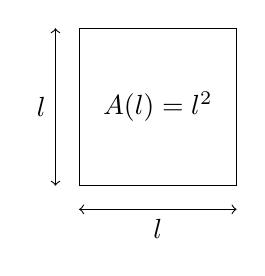
\begin{tikzpicture}
    % Draw the square
    \draw (0,0) rectangle (2,2);
    
    % Label the sides of the square
    \draw[<->] (-0.3,0) -- (-0.3,2) node[midway,left] {$l$};
    \draw[<->] (0,-0.3) -- (2,-0.3) node[midway,below] {$l$};
    
    % Label the area of the square
    \node at (1,1) {$A(l) = l^2$};
\end{tikzpicture}
\end{center}
Mathematisch wird diese Funktion gerne mit $A(.)$ benannt - der Buchstabe  $A$ stammt aus dem Englischen \emph{area} und entspricht dem Deutschen \emph{Flächeninhalt}. Die Klammern $(.)$ signalisieren, dass es sich bei $A$ um eine Funktion handelt, welche ein \textbf{Funktionsargument} aufnimmt (in diesem Fall die Seitenlänge $l$) und diesem einen \textbf{Funktionswert} zuweist (in diesem Fall das Quadrat der Seitenlänge $l^2$). Mathematisch korrekt kann man diese Funktion so definieren:
\begin{IEEEeqnarray*}{rCcCl}
  %\subnumberinglabel{eq:1}
  A &: & \mathbb{R}_{\geqslant 0} & \rightarrow & \mathbb{R}\\
  & &l &\mapsto & l^2.
\end{IEEEeqnarray*}

Das lässt sich so aussprechen: \emph{``$A$ ist eine Funktion von den nicht-negativen reellen Zahlen $(\mathbb{R}_{\geqslant 0})$, nach den reellen Zahlen  $(\mathbb{R})$. Jedem Element $l$ aus $\mathbb{R}_{\geqslant 0}$ wird das Quadrat von $l$ in $\mathbb{R}$ zugeordnet.''}
\end{example}
\begin{remark}
Manchmal wird die Definitionsmenge auch \textbf{Ursprungsmenge} und genannt. Die {Zielmenge} ist die Menge, in welcher der {Funktionswert} angenommen wird. Manchmal wird diese auch \textbf{Bildmenge} genannt.
Im Englischen spricht man von \emph{domain} für die {Definitionsmenge} und \emph{codomain} für die Zielmenge.

Das {Funktionsargument} wird auch \textbf{Funktionsvariabel} oder kurz \textbf{Variabel} genannt (um darauf aufmerksam zu machen, dass dieser Wert variieren kann).

Ein $(x,y)$ ist ein \textbf{Wertepaar} einer Funktion $f$, wenn $f(x) = y$ gilt. Im Deutschen Sprachraum wird manchmal auch die Notation $(x \mid y)$ verwendet.
\end{remark}
\newpage
\begin{exercise}
Es sei die Funktion $A$ wie aus Beispiel~\ref{ex:square}.
\begin{enumerate}[label=\alph*)]
\item Was ist die Definitionsmenge? Was ist die Zielmenge?
\item Für welche Funktionsargumente ist die Funktion definiert?
\item Berechnen Sie die Flächen der Quadrate für folgende Seitenlängen:\\[1em]
\begin{tabularx}{\linewidth} {c| *{4}{Y|} }
%\begin{tabular}{l|c|c|c|c|}
\toprule
Seitenlänge $l$ & 0~cm & 1~cm & 2~cm & 3~cm\\
\hline
Fläche $A(l)$ & \hspace{1.5cm} & \hspace{1.5cm}&\hspace{1.5cm} & 
\\[1cm]
\bottomrule
%\end{tabular}
\end{tabularx}
\item Stellen Sie die Fläche als Funktion der Seitenlänge graphisch dar:\\
\begin{center}
\begin{tikzpicture}[>=Stealth, scale=0.5]
    % Draw grid
    \draw[very thin, color=gray!30] (-6,-2) grid (6,10); % Grid lines

    % Draw axes
    \draw[->] (-6,0) -- (6,0) node[right] {\footnotesize $l$}; % x-axis
    \draw[->] (0,-2) -- (0,10) node[above] {\footnotesize $A(l)$}; % y-axis

    % Add ticks and labels on x-axis
    %\draw (0, 0) node[above left] {\tiny $0$};
    \foreach \x in {-6,...,-1}
        \draw (\x,0.1) -- (\x,-0.1) node[below] {\tiny $\x$};
    \foreach \x in {1,...,6}
        \draw (\x,0.1) -- (\x,-0.1) node[below] {\tiny $\x$};

    % Add ticks and labels on y-axis
    \foreach \y in {-2,...,-1}
        \draw (0.1,\y) -- (-0.1,\y) node[left] {\tiny $\y$};
    \foreach \y in {1,...,10}
        \draw (0.1,\y) -- (-0.1,\y) node[left] {\tiny $\y$};
\end{tikzpicture}
\end{center}
\item Gibt es Werte aus der Zielmenge, die von der Funktion nicht angenommen werden?\\
\vspace*{0.5cm}
\end{enumerate}
\end{exercise}
\newpage
\subsection{Der Unterschied zwischen der Repräsentation und dem Objekt}\label{subsubsec:notation}
Die Wahl des Buchstaben, mit dem das Funktionsargument bezeichnet wird, steht der Person offen, die die Funktion definiert. Ebenso darf diese Person den Namen der Funktion wählen. Im obigen Beispiel hätte man die Funktion selbst auch mit $\texttt{Fläche}(.)$ benennen können und das Argument mit $\texttt{Länge}$:
\begin{IEEEeqnarray*}{rCcCl}
  %\subnumberinglabel{eq:1}
  \texttt{Fläche} &: & \mathbb{R} & \rightarrow & \mathbb{R}\\
  & &\texttt{Länge} &\mapsto & \left(\texttt{Länge}\right)^2.
\end{IEEEeqnarray*}

Es liegt nahe, Funktionen und deren Argumente mit einzelnen Buchstaben zu bezeichnen, um den Text übersichtlich zu gestalten. Häufige Buchstaben zur Bezeichnung von Funktionen sind $f,g$ und $h$. Funktionsargumente werden häufig mit den folgenden Buchstaben beschrieben:

\begin{itemize}
\item $t$, wenn es sich um zeitliche Grössen handelt (vom Englischen \emph{time});
\item $n$, wenn es sich um diskrete (zählbare) Grössen handelt (vom Englischen \emph{number}, im Sinne einer ganzen Zahl);
\item $x,y,z$, wenn mit einem kartesischen Koordinatensystem gearbeitet wird (um Grössen der $x, y$ oder $z$ -Koordinaten zu beschreiben);
\item $\theta$, wenn es sich um Winkel handelt.
\end{itemize}

Bedenken Sie, dass diese Buchstaben immer nur eine \textbf{Repräsentation} des mathematischen Objektes sind. In Beispiel~\ref{ex:square} steht $l$ repräsentativ für \emph{ein Element aus der Definitionsmenge}. Die Funktion nimmt nicht den Buchstaben ``$l$'' als Argument, sondern das Element, das durch $l$ repräsentiert wird.

In Aufgabe~\ref{ex:func_definitions} haben Sie Gelegenheit, Ihr Abstraktionsvermögen zu trainieren: Entdecken Sie, welche Schreibweisen das gleiche mathematische Objekt repräsentieren?
\begin{remark}\label{rem:implicit_def}
Häufig werden Funktionen gerne etwas kompakter beschrieben. So liesse sich die Funktion $A$ aus Beispiel~\ref{ex:square} auch folgendermassen umschreiben:
\begin{IEEEeqnarray*}{rClR}
  %\subnumberinglabel{eq:1}
  A(l) &= l^2, &\forall \; l \in \mathbb{R}_{\geqslant 0}.
\end{IEEEeqnarray*}
Dies liest sich als \emph{``A von $l$ ist gleich $l$ hoch zwei für jedes $l$ der nicht-negativen reellen Zahlen.''}.

Diese Art der Definition ist allerdings \textbf{ungenau}, da die {Zielmenge} nicht explizit definiert ist!

In Beispiel~\ref{ex:square} ist die Zielmenge die Menge \emph{aller} reellen Zahlen. Aber was ist sie hier? die Menge aller reellen Zahlen? Die Menge aller nicht-negativen reellen Zahlen? Die Menge aller nicht-negativen reellen Zahlen und die Menge aller Äpfel, die Im Jahr 1913 im Thurgau produziert wurden?

Um Ungenauigkeiten zu vermeiden, müssen deshalb immer Definitionsmenge \emph{und} Zielmenge definiert werden. In Kapitel~\ref{subsubsec:eindeutigkeit} wird dieses Thema nochmals aufgegriffen.
\end{remark}

\begin{exercise}\label{ex:func_definitions}
Welche der folgenden Definitionen beschreiben die gleiche Funktion?
\begin{enumerate}[2col, label=\alph*)]
\footnotesize
\item \begin{IEEEeqnarray*}{rCcCl}
  %\subnumberinglabel{eq:1}
  f &: & \mathbb{R} & \rightarrow & \mathbb{R}\\
  & &x &\mapsto & x^2.
\end{IEEEeqnarray*}
\item \begin{IEEEeqnarray*}{rCcCl}
  %\subnumberinglabel{eq:1}
  g &: & \mathbb{R} & \rightarrow & \mathbb{R}\\
  & &\theta &\mapsto & 3\theta +3.
\end{IEEEeqnarray*}

\item \begin{IEEEeqnarray*}{rCcCl}
  %\subnumberinglabel{eq:1}
  h &: & \mathbb{R} & \rightarrow & \mathbb{R}\\
  & &y &\mapsto & y^2.
\end{IEEEeqnarray*}
\item \begin{IEEEeqnarray*}{rCcCl}
  %\subnumberinglabel{eq:1}
  r &: & \mathbb{R} & \rightarrow & \mathbb{R}\\
  & &z &\mapsto & 3(z+1).
\end{IEEEeqnarray*}
\item \begin{IEEEeqnarray*}{rCcCl}
  %\subnumberinglabel{eq:1}
  K &: & \mathbb{R} & \rightarrow & \mathbb{R}\\
  & &t &\mapsto & 3t +3.
\end{IEEEeqnarray*}
\item \begin{IEEEeqnarray*}{rCcCl}
  %\subnumberinglabel{eq:1}
  \blacktriangle &: & \mathbb{R} & \rightarrow & \mathbb{R}\\
  & &v &\mapsto & v^2.
\end{IEEEeqnarray*}
\item \begin{IEEEeqnarray*}{rCcCl}
  %\subnumberinglabel{eq:1}
  \blacksquare &: & \mathbb{R} & \rightarrow & \mathbb{R}\\
  & &\blacklozenge &\mapsto & 3\blacklozenge +3.
\end{IEEEeqnarray*}
\item \begin{IEEEeqnarray*}{rCcCl}
  %\subnumberinglabel{eq:1}
  \nabla &: & \mathbb{R} & \rightarrow & \mathbb{R}\\
  & &\spadesuit &\mapsto & \spadesuit^2.
\end{IEEEeqnarray*}
\item \begin{IEEEeqnarray*}{rCcCl}
  %\subnumberinglabel{eq:1}
  \bigstar &: & \mathbb{R} & \rightarrow & \mathbb{R}\\
  & &\blacktriangledown\square\spadesuit &\mapsto & \left(\blacktriangledown\square\spadesuit\right)^2 +1 -1.
\end{IEEEeqnarray*}
\item \begin{IEEEeqnarray*}{rCcCl}
  %\subnumberinglabel{eq:1}
  \S &: & \mathbb{R} & \rightarrow & \mathbb{R}\\
  & &\blacklozenge &\mapsto & 3\blacklozenge +3.
\end{IEEEeqnarray*}
\end{enumerate}
\vspace*{1cm}
\end{exercise}


\subsection{Eindeutigkeiten von Funktionen}\label{subsubsec:eindeutigkeit}
Ihnen ist vielleicht aufgefallen, dass die Definition einer Funktion verlangt, dass sie \emph{jedem} Element der Definitionsmenge \emph{genau ein} Element der Zielmenge zuordnet. Es ist aber durchaus möglich, dass die Funktion mehreren Elementen der Definitionsmenge das gleiche Element aus der Zielmenge zuordnet, und einem oder mehreren Elementen der Zielmenge kein Element zuordnet.

In der Mathematik wird dieses Verhalten einer Funktion mit spezifischen Begriffen bezeichnet. Man spricht von \emph{injektiven}, \emph{surjektiven} oder \emph{bijektiven} Funktionen.
\begin{figure}[ht]
\centering

\begin{subfigure}[t]{0.3\textwidth}
\centering
% Injective
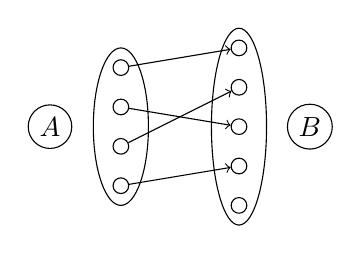
\begin{tikzpicture}[scale=0.5, every node/.style={circle,draw,inner sep=2pt}, baseline=(current bounding box.center)]
    % Ellipse for Set A
    \node (a1) at (0,1) {};
    \node (a2) at (0,0) {};
    \node (a3) at (0,-1) {};
    \node (a0) at (0,-2) {};
    \draw (0,-0.5) ellipse (0.7cm and 2cm) node[xshift=-0.9cm] {$A$};

    % Ellipse for Set B
    \node (b0) at (3,1.5) {};
    \node (b1) at (3,0.5) {};
    \node (b2) at (3,-0.5) {};
    \node (b3) at (3,-1.5) {};
    \node (b4) at (3,-2.5) {};
    \draw (3,-0.5) ellipse (0.7cm and 2.5cm) node[xshift=0.9cm] {$B$};

    % Arrows
    \draw[->] (a0) -- (b3);
    \draw[->] (a1) -- (b0);
    \draw[->] (a2) -- (b2);
    \draw[->] (a3) -- (b1);
\end{tikzpicture}
\caption{injektiv, nicht surjektiv}
\end{subfigure}
%
\hfill % Adds horizontal space between figures
%
\begin{subfigure}[t]{0.3\textwidth}
\centering
% Surjective
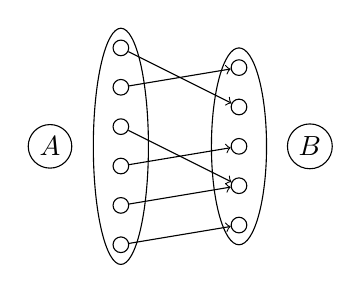
\begin{tikzpicture}[scale=0.5, every node/.style={circle,draw,inner sep=2pt}, baseline=(current bounding box.center)]
    % Ellipse for Set A
    \node (a6) at (0,2) {};
    \node (a1) at (0,1) {};
    \node (a2) at (0,0) {};
    \node (a3) at (0,-1) {};
    \node (a0) at (0,-2) {};
    \node (a5) at (0, -3) {};
    \draw (0,-0.5) ellipse (0.7cm and 3cm) node[xshift=-0.9cm] {$A$};

    % Ellipse for Set B
    \node (b0) at (3,1.5) {};
    \node (b1) at (3,0.5) {};
    \node (b2) at (3,-0.5) {};
    \node (b3) at (3,-1.5) {};
    \node (b4) at (3,-2.5) {};
    \draw (3,-0.5) ellipse (0.7cm and 2.5cm) node[xshift=0.9cm] {$B$};

    % Arrows
    \draw[->] (a6) -- (b1);
    \draw[->] (a0) -- (b3);
    \draw[->] (a1) -- (b0);
    \draw[->] (a2) -- (b3);
    \draw[->] (a3) -- (b2);
    \draw[->] (a5) -- (b4);
\end{tikzpicture}
\caption{surjektiv, nicht injektiv}
\end{subfigure}
%
\hfill % Adds horizontal space between figures
%
\begin{subfigure}[t]{0.3\textwidth}
\centering
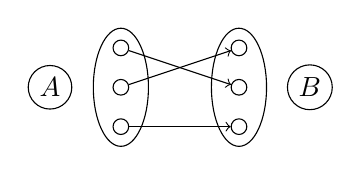
\begin{tikzpicture}[scale=0.5, every node/.style={circle,draw,inner sep=2pt}, baseline=(current bounding box.center)]
    % Ellipse for Set A
    \node (a1) at (0,1) {};
    \node (a2) at (0,0) {};
    \node (a3) at (0,-1) {};
    \draw (0,0) ellipse (0.7cm and 1.5cm) node[xshift=-0.9cm] {$A$};

    % Ellipse for Set B
    \node (b1) at (3,1) {};
    \node (b2) at (3,0) {};
    \node (b3) at (3,-1) {};
    \draw (3,0) ellipse (0.7cm and 1.5cm) node[xshift=0.9cm] {$B$};

    % Arrows
    \draw[->] (a1) -- (b2);
    \draw[->] (a2) -- (b1);
    \draw[->] (a3) -- (b3);
\end{tikzpicture}
\caption{bijektiv}
\end{subfigure}
\caption{Ikonische Darstellung von Injektivität, Surjektivität und Bijektivität}\label{fig:injective}
\end{figure}

\begin{exercise}\label{ex:func_behavior}
\begin{enumerate}[label=\alph*)]
\item Betrachten Sie Abbildung~\ref{fig:injective} auf Seite~\pageref{fig:injective}. Was bedeutet es Ihrer Meinung nach, wenn eine Funktion \emph{injektiv}, \emph{surjektiv} oder \emph{bijektiv} ist? Schreiben Sie hier eine Definition für jeden der drei Begriffe auf.\\
\vspace*{5cm}
\item Gibt es Unterschiede zwischen Ihrer Definition und Definition~\ref{def:injectivity} auf Seite~\pageref{def:injectivity}?
\vspace*{3cm}
\end{enumerate}
\end{exercise}
\newpage
\begin{whitebox}
\begin{definition}\label{def:injectivity}
\begin{enumerate}[label=\alph*)]
\item Eine Funktion ist \textbf{injektiv}, wenn jedes Element der Zielmenge \textbf{höchstes} ein Urbild hat. Sprich, eine Funktion  $f: A \rightarrow B$ ist injektiv, wenn für alle $x_1, x_2 \in A$, so dass $x_1\neq x_2$, gilt $f(x_1) \neq f(x_2)$.
\item Eine Funktion ist \textbf{surjektiv}, wenn jedes Element der Zielmenge \textbf{mindestens} ein Urbild hat. Sprich, eine Funktion $f: A \rightarrow B$ ist \textbf{surjektiv}, wenn für jedes $y \in B$, mindestens ein $x\in A$ existiert, so dass $f(x) = y$.
\item Eine Funktion ist \textbf{bijektiv}, wenn sie \textbf{injektiv und surjektiv} ist. Mit anderen Worten: für jedes Element der Zielmenge, gibt es genau ein Urbild. Sprich, eine Funktion $f: A \rightarrow B$ ist surjektiv, wenn für jedes $y \in B$, genau ein $x\in A$ existiert, so dass $f(x) = y$.
\end{enumerate}
\end{definition}
\end{whitebox}

\begin{remark}
Anstatt \emph{injektiv} sagt man auch \textbf{linkseindeutig}.
\end{remark}

\begin{exercise}\label{ex:class_injektiv_surjektiv_bijektiv}
Bestimmen Sie für jede der folgenden Funktionen, ob diese injektiv, surjektiv oder bijektiv ist:
\begin{enumerate}[2col, label=\alph*)]
\item \begin{IEEEeqnarray*}{rCcCl}
  %\subnumberinglabel{eq:1}
  f &: & \mathbb{R} & \rightarrow & \mathbb{R}\\
  & &x &\mapsto & x.
\end{IEEEeqnarray*}
\item \begin{IEEEeqnarray*}{rCcCl}
  %\subnumberinglabel{eq:1}
  g &: & \mathbb{R} & \rightarrow & \mathbb{R}\\
  & &z &\mapsto & z^2.
\end{IEEEeqnarray*}
\item \begin{IEEEeqnarray*}{rCcCl}
  %\subnumberinglabel{eq:1}
  h &: & \mathbb{R}_{\geqslant 0} & \rightarrow & \mathbb{R}\\
  & &y &\mapsto & y^2.
\end{IEEEeqnarray*}
\item \begin{IEEEeqnarray*}{rCcCl}
  %\subnumberinglabel{eq:1}
  w &: & \mathbb{R} & \rightarrow & \mathbb{R}\\
  & &t &\mapsto & 2t^2.
\end{IEEEeqnarray*}
\item \begin{IEEEeqnarray*}{rCcCl}
  %\subnumberinglabel{eq:1}
  v &: & \mathbb{R}_{\geqslant 0} & \rightarrow & \mathbb{R}_{\geqslant 0}\\
  & &x &\mapsto & x^2.
\end{IEEEeqnarray*}
\item \begin{IEEEeqnarray*}{rCcCl}
  u &: & \mathbb{R} & \rightarrow & \mathbb{R}\\
  & &t &\mapsto & 4t+2
\end{IEEEeqnarray*}
\end{enumerate}
\vspace*{0.45cm}
\end{exercise}

\subsection{Operationen mit Funktionen}
Man darf Operationen wie Addition, Subtraktion, Multiplikation und Division mit Funktionen durchführen, wenn die Definitionsmengen dies zulassen.

\subsubsection{Addition und Subtraktion}
\begin{example}\label{exmpl:operationen_mit_funktionen}
Es seien die Funktionen $f$ und $g$ wie folgt definiert:
\begin{IEEEeqnarray*}{rCrClCrCrCl}
f &:& \mathbb{R} &\rightarrow& \mathbb{R}, &\qquad \qquad& g &:& \mathbb{R} &\rightarrow & \mathbb{R}\\
&& x&\mapsto& -2x+5 & &&& y &\mapsto& 0.5y-10
\end{IEEEeqnarray*}
Dann ist die Summe $f+g$ beider Funktionen wiederum eine Funktion:
\begin{IEEEeqnarray*}{rCrCl}
(f+g) & : & \mathbb{R} & \rightarrow \mathbb{R}\\
&& x &\mapsto& (-2x + 5) + (0.5x -10) = -1.5x -5
\end{IEEEeqnarray*}
Gleich kann man mit $f-g$ und sogar $f\cdot g$ verfahren.

\begin{center}
\resizebox{0.7\textwidth}{!}{
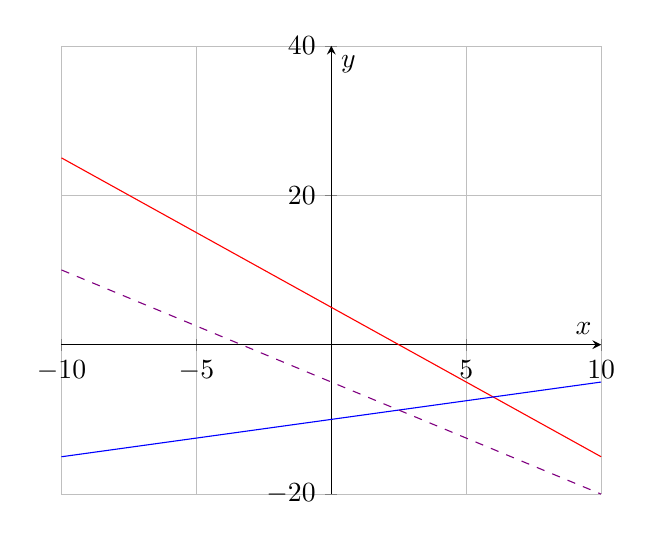
\begin{tikzpicture}
\begin{axis}[
    axis lines=center,
    xlabel={$x$},
    ylabel={$y$},
    xmin=-10, xmax=10,
    ymin=-20, ymax=40,
    %legend pos=outer north east,
    %title={Funktionsgraph von $f(x) = -2x + 1$, $g(x) = 0.5x -2$ und ihren linearen Kombinationen},
    clip=false,
    grid=both,
    grid style={line width=.1pt, draw=gray!10},
    major grid style={line width=.2pt,draw=gray!50},
]
% f(x) = -2x + 4
\addplot[domain=-10:10, samples=100, red] {-2*x + 5};
%\addlegendentry{$f(x) = -2x + 5$}
% g(x) = x^2 + 1
\addplot[domain=-10:10, samples=100, blue] {0.5*x-10};
%\addlegendentry{$g(x) = 0.5x-10$}
% f+g
\addplot[domain=-10:10, samples=100, violet, dashed] {0.5*x-10 + -2*x + 5};
%\addlegendentry{$f+g$}
% f*g
%\addplot[domain=-3:3, samples=100, orange, dashdotted] {(-2*x + 1) * (0.5*x-2)};
%\addlegendentry{$f \cdot g$}
% f-g
%\addplot[domain=-10:10, samples=100, green!50!black, densely dotted] {-2*x + 5 - (0.5*x-10)};
%\addlegendentry{$f-g$}
\end{axis}
\end{tikzpicture}
}
\end{center}
\end{example}


\begin{whitebox}
\begin{definition}
Es seien $f : A \rightarrow \mathbb{R}$ und $g:B \rightarrow \mathbb{R}$ zwei Funktionen, dann gilt:

\textbf{Addition zweier Funktionen:}
$f+g$ ist wiederum eine Funktion, mit Definitionsmenge $A \cap B$ und Zielmenge $\mathbb{R}$, definiert als:
\begin{IEEEeqnarray*}{rCrCl}
(f+g) & : & A \cap B &\rightarrow& \mathbb{R}\\
& & x &\mapsto& f(x) + g(x)
\end{IEEEeqnarray*}

\textbf{Subtraktion zweier Funktionen:}
$f-g$ ist wiederum eine Funktion, mit Definitionsmenge $A \cap B$ und Zielmenge $\mathbb{R}$, definiert als:
\begin{IEEEeqnarray*}{rCrCl}
(f-g) & : & A \cap B &\rightarrow& \mathbb{R}\\
& & x &\mapsto& f(x) - g(x)
\end{IEEEeqnarray*}
\end{definition}
\end{whitebox}

\begin{remark}
$A \cap B$ ist die Schnittmenge der Menge $A$ mit der Menge $B$, sie auch Seite~\pageref{terminologie}.
\end{remark}



\begin{exercise}\label{ex:einfuehrung_lin_comb_func}
\begin{enumerate}[label=\alph*)]
\item Es seien $f$ und $g$ wie in Beispiel~\ref{exmpl:operationen_mit_funktionen}.
\begin{enumerate}[label=\roman*)]
\item Welcher der Graphen aus Beispiel~\ref{exmpl:operationen_mit_funktionen} gehört zu $f$, welcher zu $g$, welcher zu $f+g$? Schreiben Sie die Graphen an.
\item Definieren Sie die Funktion $f-g$ und zeichnen Sie diese in den Graphen ein.
\end{enumerate} 
\item Es seien $v$ und $u$ zwei Funktionen wie folgt definiert:
\begin{IEEEeqnarray*}{rCrClCrCrCl}
v &:& ]-\infty, -1[ \cup [1, +\infty[ &\rightarrow& \mathbb{R}, &\qquad \qquad& u &:& \mathbb{R} &\rightarrow & \mathbb{R}\\
&& x&\mapsto&  \frac{1}{x} & &&& y &\mapsto& 1+y
\end{IEEEeqnarray*}
\begin{enumerate}[label=\roman*)]
\item Definieren Sie die Funktion $v+u$.
\item Definieren Sie die Funktion $v-u$.
\item Was passiert mit dem Funktionswert von $v$, wenn man den Definitionsbereich auf das Intervall $\mathbb{R} \setminus \{0\}$ ausweiten würde?
\end{enumerate}
\end{enumerate}
\end{exercise}

\subsubsection{Multiplikation und Division}
Man darf Funktionen auch miteinander multiplizieren und sogar dividieren (allerdings mit viel Sorgfalt!).
\begin{example}\label{exmpl: funktionen_multiplikation}
Es seien $f$ und $g$ wie aus dem Beispiel~\ref{exmpl:operationen_mit_funktionen}, dann sind folgende Funktionen gut definiert:
\begin{IEEEeqnarray*}{rCrClCrCrCl}
(f \cdot g) &:& \mathbb{R} &\rightarrow& \mathbb{R}, &\qquad \qquad& \left(\frac{f}{g}\right) & : & \mathbb{R}\setminus\left\{20\right\} &\rightarrow& \mathbb{R}\\
& & x &\mapsto& f(x) \cdot g(x) & &&& x &\mapsto& \frac{f(x)}{g(x)}
\end{IEEEeqnarray*}

\begin{center}
\resizebox{0.7\textwidth}{!}{
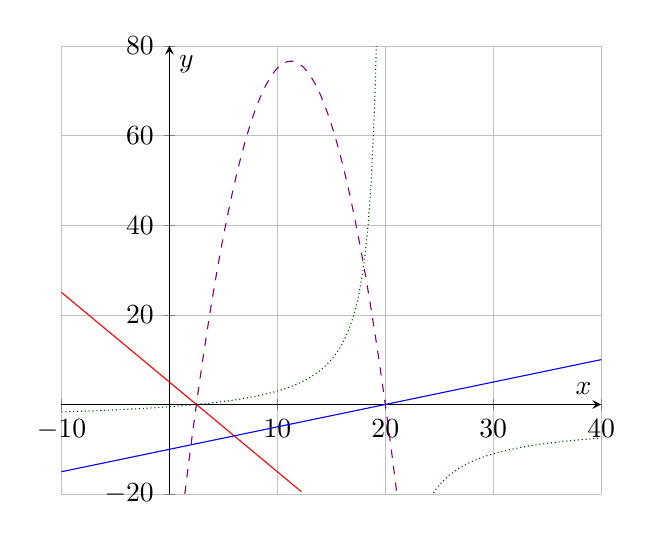
\begin{tikzpicture}
\begin{axis}[
    axis lines=center,
    xlabel={$x$},
    ylabel={$y$},
    xmin=-10, xmax=40,
    ymin=-20, ymax=80,
    %legend pos=outer north east,
    %title={Funktionsgraph von $f(x) = -2x + 1$, $g(x) = 0.5x -2$ und ihren linearen Kombinationen},
    restrict y to domain=-20:80,
    clip=false,
    grid=both,
    grid style={line width=.1pt, draw=gray!10},
    major grid style={line width=.2pt,draw=gray!50},
]
% f(x) = -2x + 4
\addplot[domain=-10:40, samples=100, red] {-2*x + 5};
%\addlegendentry{$f(x) = -2x + 5$}
% g(x) = x^2 + 1
\addplot[domain=-10:40, samples=100, blue] {0.5*x-10};
%\addlegendentry{$g(x) = 0.5x-10$}
% f+g
\addplot[domain=-0:25, samples=1000, violet, dashed] {(0.5*x-10 )* (-2*x + 5)};
%\addlegendentry{$f+g$}
% f*g
%\addplot[domain=-3:3, samples=100, orange, dashdotted] {(-2*x + 1) * (0.5*x-2)};
%\addlegendentry{$f \cdot g$}
% f-g

\addplot[domain=-10:19, samples=100, green!30!black, densely dotted] {(-2*x + 5)/(0.5*x-10 )};
\addplot[domain=21:40, samples=100, green!30!black, densely dotted] {(-2*x + 5)/(0.5*x-10 )};
\addplot[domain=19:21, samples=1000, green!30!black, densely dotted] {(-2*x + 5)/(0.5*x-10 )};
%\addlegendentry{$f-g$}
\end{axis}
\end{tikzpicture}
}
\end{center}
\end{example}
\begin{whitebox}
\begin{definition}
Es seien $f : A \rightarrow \mathbb{R}$ und $g:B \rightarrow \mathbb{R}$ zwei Funktionen, dann gilt:

\textbf{Multiplikation zweier Funktionen:}
$f \cdot g$ ist wiederum eine Funktion, mit Definitionsmenge $A \cap B$ und Zielmenge $\mathbb{R}$, definiert als:
\begin{IEEEeqnarray*}{rCrCl}
(f \cdot g) & : & A \cap B &\rightarrow& \mathbb{R}\\
& & x &\mapsto& f(x) \cdot g(x)
\end{IEEEeqnarray*}

\textbf{Quotient zweier Funktionen:}
Es sei $\{x \in B \mid g(x) = 0\}$ die Menge aller Punkte von $B$, in denen $g$ den Funktionswert Null annimmt. Dann ist $\frac{f}{g}$ wie folgt definiert:
\begin{IEEEeqnarray*}{rCrCl}
\left(\frac{f}{g}\right) & : & A \cap B \setminus \{x \in B \mid g(x) = 0\} &\rightarrow& \mathbb{R}\\
& & x &\mapsto& \frac{f(x)}{g(x)}
\end{IEEEeqnarray*}
\end{definition}
\end{whitebox}
\begin{remark}
Die Menge $\{x \in B \mid g(x) = 0\}$ entspricht allen Werten $x$ aus der Menge $B$, für welche $g(x)$ gleich null ist.

Die Schreibweise mit dem Senkrechten Strich lässt sich ungefähr so lesen: $\{\textit{Startmenge} \mid \textit{Bedingung}\}$


Der erste Teil in der Mengenklammer, vor dem senkrechten Strich $\mid$ beschreibt jeweils die Menge aller Elemente, welche in Frage kommen. In diesem Fall sind das alle $x$ aus der Menge $B$. Der zweite Teil in der Mengenklammer, nach dem senkrechten Strich $\mid$ beschreibt jeweils eine \textbf{Bedingung}, die erfüllt sein muss, damit $x$ in der Menge bleiben darf.

Anbei ein Paar Beispiele: \begin{itemize}
\item $\{x \in A  \mid x \neq B \}$ : alle Elemente aus $A$, welche nicht gleichzeitig ein Element in $B$ sind. Das ist äquivalent zu der Menge $A \setminus B$
\item $\{x \in A \mid x \in B \}$: alle Elemente aus $A$, die gleichzeitig ein Element aus $B$ sind. Das ist äquivalent zu der Menge $A \cap B$
\item $\{x \in \mathbb{R} \mid x = 0\}$: alle Elemente aus $\mathbb{R}$, die gleich Null sind. Diese Menge ist gleich der Menge $\{0\}$
\item $\{x \in \mathbb{R} \mid x \geqslant 0\}$: alle Elemente aus $\mathbb{R}$, welche grösser oder gleich null sind.
\end{itemize}
Falls Sie den Umgang mit dieser Notation und Mengen im allgemeinen noch etwas üben möchten, melden Sie sich bitte bei mir und ich werde weitere Übungsaufgaben und Beispiele verfassen.
\end{remark}


\begin{exercise}
Es seien $f$ und $g$ wie in Beispiel~\ref{exmpl: funktionen_multiplikation}.
\begin{enumerate}[label=\alph*)]
\item Bestimmen Sie die Formel für die Funktion $f \cdot g$
\item Bestimmen Sie die Formel für die Funktion $\frac{f}{g}$
\item Ordnen Sie die abgebildeten Funktionsgraphen in Beispiel~\ref{exmpl: funktionen_multiplikation} den vier Funktionen $f$, $g$, $f \cdot g$ und $\frac{f}{g}$ zu.
\item Es seien $v$ und $u$ zwei Funktionen wie folgt definiert:
\begin{IEEEeqnarray*}{rCrClCrCrCl}
v &:& \mathbb{R}\setminus \{0\} &\rightarrow& \mathbb{R}, &\qquad \qquad& u &:& \mathbb{R} &\rightarrow & \mathbb{R}\\
&& x&\mapsto&  \frac{1}{x} & &&& y &\mapsto& 1+y
\end{IEEEeqnarray*}
\begin{enumerate}[label=\roman*)]
\item Bestimmen Sie $u \cdot v$
\item Bestimmen Sie $\frac{u}{v}$
\item Bestimmen Sie $\frac{v}{u}$
\end{enumerate}
\end{enumerate}
\end{exercise}


\subsubsection{Verkettung}
Funktionen dürfen auch miteinander \emph{verkettet} werden.
\begin{example}\label{exmpl:func_verkettung}
Es seien $f$ und $g$ zwei Funktionen definiert als:
\begin{IEEEeqnarray*}{rCrClCrCrCl}
f &:& \mathbb{R}\setminus \{0\} &\rightarrow& \mathbb{R}, &\qquad \qquad& g &:& \mathbb{R} &\rightarrow & \mathbb{R}\\
&& x&\mapsto&  \frac{1}{x} & &&& y &\mapsto& 1-y
\end{IEEEeqnarray*}

Dann kann ich $f$ und $g$ folgendermassen \emph{verketten}:
\begin{IEEEeqnarray*}{rCrCl}
g \circ f &:& \mathbb{R} &\rightarrow& \mathbb{R}\\
&& x &\mapsto & g(f(x))
\end{IEEEeqnarray*}

Das heisst, der Funktionswert von $f$ im Punkt $x$ wird mein Funktionsargument für $g$. Das lässt sich noch weiter ausschreiben: $g(f(x)) = 1-\frac{1}{x}$

\begin{center}
\resizebox{0.7\textwidth}{!}{
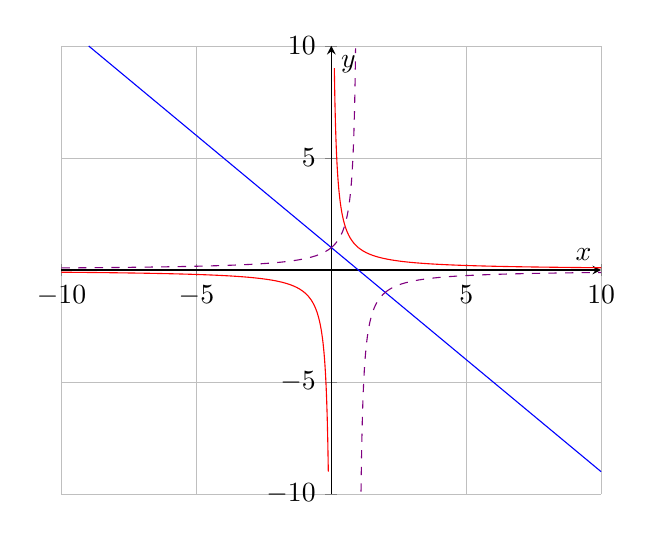
\begin{tikzpicture}
\begin{axis}[
    axis lines=center,
    xlabel={$x$},
    ylabel={$y$},
    xmin=-10, xmax=10,
    ymin=-10, ymax=10,
    %legend pos=outer north east,
    %title={Funktionsgraph von $f(x) = -2x + 1$, $g(x) = 0.5x -2$ und ihren linearen Kombinationen},
    restrict y to domain=-10:10,
    clip=false,
    grid=both,
    grid style={line width=.1pt, draw=gray!10},
    major grid style={line width=.2pt,draw=gray!50},
]
% f(x) = -2x + 4
\addplot[domain=-10:-1, samples=100, red] {1/x};
\addplot[domain=-1:1, samples=100, red] {1/x};
\addplot[domain=1:10, samples=100, red] {1/x};
\addplot[domain=-10:10, samples=100, blue] {1-x};
\addplot[domain=-10:0, samples=1000, violet, dashed] {1/(1-x)};
\addplot[domain=0:2, samples=1000, violet, dashed] {1/(1-x)};
\addplot[domain=2:10, samples=1000, violet, dashed] {1/(1-x)};
%\addlegendentry{$f-g$}
\end{axis}
\end{tikzpicture}
}
\end{center}
\end{example}


\begin{whitebox}
\begin{definition}
In der Mathematik spricht man von einer \textbf{Funktionsverknüpfung}, \textbf{Funktionsverkettung} oder \textbf{Komposition}, wenn mehrere Funktionen miteinander verknüpft werden, indem der Funktionswert der einen Funktion als Funktionsargument in der nächsten Funktion genutzt wird.

Wenn $f: A \rightarrow B$ und $g: B \rightarrow C$ zwei Funktionen sind, so kann man diese wie folgt verknüpfen:
\begin{IEEEeqnarray*}{rCrCl}
g \circ f &:& A &\rightarrow& C\\
&& x &\mapsto & g(f(x))
\end{IEEEeqnarray*}

$f$ ist in diesem Fall die \textbf{innere Funktion}, während $g$ als die \textbf{äussere Funktion} bezeichnet wird.
\end{definition}
\end{whitebox}

\begin{remark}
Bei der Funktionsverkettung wie auch anderen Operationen zwischen Funktionen, muss man darauf Acht geben, dass die Definitionsmengen eingehalten werden. \textbf{Die Zielmenge der inneren Funktion muss immer komplett in der Definitionsmenge der äusseren Funktion enthalten sein}, ansonsten riskiert man, schlecht definierte Funktionen zu erhalten.

Das kann an folgendem Beispiel verdeutlicht werden. Es seien $f$ und $g$ wie folgt:
\begin{IEEEeqnarray*}{rCrClCrCrCl}
f &:& \mathbb{R} \setminus \{0\} &\rightarrow& \mathbb{R}, &\qquad \qquad& g &:& \mathbb{R} &\rightarrow & \mathbb{R}\\
&& x&\mapsto&  \frac{1}{x} & &&& y &\mapsto& y+1
\end{IEEEeqnarray*}
Offensichtlich darf man die Funktion $g \circ f$ konstruieren, da die Zielmenge $\mathbb{R}$ von $f$ komplett in der Definitionsmenge von $g$ enthalten ist.


Allerdings muss man aufpassen, wenn man die Reihenfolge der Verkettung ändert. Die Zielmenge von $g$ enthält die Zahl Null. \textbf{Wenn man die Definitionsmenge nicht anpasst, riskiert man, durch Null zu dividieren!} Man muss darum $\{-1\}$ aus der Definitionsmenge ausschliessen:
\begin{IEEEeqnarray*}{lCrCl}
f \circ g &:& \mathbb{R} \setminus \{-1\} &\rightarrow &\mathbb{R}\\
&& x &\mapsto & \frac{1}{x+1}
\end{IEEEeqnarray*}
\end{remark}

\begin{exercise}
Es seien $f$ und $g$ wie aus Beispiel~\ref{exmpl:func_verkettung}
\begin{enumerate}[label=\alph*)]
\item Ordnen Sie die abgebildeten Funktionsgraphen in Beispiel~\ref{exmpl:func_verkettung} den drei Funktionen $f$, $g$ und $g \circ f$ zu.
\item Dürfen Sie die Verknüpfungsfolge ändern? Also mit $f \circ g$ anstatt $g \circ f$ arbeiten?
\end{enumerate}
\end{exercise}

\begin{exercise}
\begin{enumerate}[label=\alph*)]
\item Es seien $v$ und $u$ zwei Funktionen wie folgt definiert:
\begin{IEEEeqnarray*}{rCrClCrCrCl}
v &:& \mathbb{R}\setminus\{-1\} &\rightarrow& \mathbb{R}, &\qquad \qquad& u &:& \mathbb{R} &\rightarrow & \mathbb{R}\\
&& x&\mapsto&  \frac{1}{x+1} & &&& y &\mapsto& 4+3y
\end{IEEEeqnarray*}
\begin{enumerate}[label=\roman*)]
\item Ist die Funktion $u \circ v$ gut definiert? Was ist die Definitionsmenge? Was ist die Zielmenge? Was ist der Funktionswert im Punkt $5$?
\item Können Sie die Definitionsmenge so anpassen, dass die Funktion $v \circ u$ gut definiert ist?
\end{enumerate}
\end{enumerate}
\end{exercise}

\newpage
\subsection{Übungen}
\begin{exercise}\label{ex:schlecht_definiert}
Welche dieser Funktionen sind gut definiert? Welche sind schlecht definiert?
\begin{enumerate}[2col, label=\roman*)]
\item \begin{IEEEeqnarray*}{rCcCl}
  f &: & \mathbb{R} & \rightarrow & \mathbb{R}_{+}\\
  & &x &\mapsto & x^2
\end{IEEEeqnarray*}
\item \begin{IEEEeqnarray*}{rCcCl}
  g &: & [0,2] & \rightarrow & [0,1]\\
  & &x &\mapsto & x^2
\end{IEEEeqnarray*}
\item \begin{IEEEeqnarray*}{rCcCl}
  v &: & \mathbb{R}_{\geqslant 0} & \rightarrow & \mathbb{R}\\
  & &t &\mapsto & 4t+10
\end{IEEEeqnarray*}
\item \begin{IEEEeqnarray*}{rCcCl}
  \bigstar &: & [0,1] & \rightarrow & [1,2]\\
  & &x &\mapsto & x^2 + 1
\end{IEEEeqnarray*}
\columnbreak
\item  \begin{IEEEeqnarray*}{rCcCl}
  h &: & \lbrace \clubsuit, \diamondsuit, \heartsuit, \spadesuit \rbrace & \rightarrow & \lbrace 0,1,2,3\rbrace\\
  & &\clubsuit &\mapsto & 0\\
  & &\diamondsuit &\mapsto & 1\\
  & &\heartsuit &\mapsto & 2\\
  & &\spadesuit &\mapsto & 3\\
\end{IEEEeqnarray*}
\item  \begin{IEEEeqnarray*}{rCcCl}
  w &: & \lbrace \clubsuit, \diamondsuit, \heartsuit, \spadesuit \rbrace & \rightarrow & \lbrace 0,1,2,3\rbrace\\
  & &\clubsuit &\mapsto & 0\\
  & &\diamondsuit &\mapsto & 1\\
  & &\clubsuit &\mapsto & 2\\
  & &\spadesuit &\mapsto & 3\\
\end{IEEEeqnarray*}
\item \begin{IEEEeqnarray*}{rCcCl}
  u &: & \mathbb{R} & \rightarrow & \mathbb{R}_{\geqslant 0}\\
  & &x &\mapsto & x^2
\end{IEEEeqnarray*}
\end{enumerate}\hfill\\
\end{exercise}
\newpage
\begin{exercise}\label{ex:injektiv_surjektiv_bijektiv}
Bestimmen Sie für jede dieser Funktionen, ob sie injektiv, surjektiv oder bijektiv ist.
\begin{enumerate}[2col, label=\roman*)]
\item \begin{IEEEeqnarray*}{rCcCl}
  f &: & [0,1] & \rightarrow & [-1,4]\\
  & &x &\mapsto & x^2
\end{IEEEeqnarray*}
\item \begin{IEEEeqnarray*}{rCcCl}
  g &: & \mathbb{R} & \rightarrow & \mathbb{R}\\
  & &x &\mapsto & 2x + 1
\end{IEEEeqnarray*}
\item \begin{IEEEeqnarray*}{rCcCl}
  w &: & [-1,1] & \rightarrow & \mathbb{R}\\
  & &x &\mapsto & x^2
\end{IEEEeqnarray*}
\item \begin{IEEEeqnarray*}{rCcCl}
  v &: & \mathbb{R}_{\geqslant 0} & \rightarrow & \mathbb{R}\\
  & &t &\mapsto & 4t+10
\end{IEEEeqnarray*}
\item \begin{IEEEeqnarray*}{rCcCl}
  \bigstar &: & [0,1] & \rightarrow & [1,2]\\
  & &x &\mapsto & x^2 + 1
\end{IEEEeqnarray*}
\item  \begin{IEEEeqnarray*}{rCcCl}
  h &: & \lbrace \clubsuit, \diamondsuit, \heartsuit, \spadesuit \rbrace & \rightarrow & \lbrace 0,1,2,3\rbrace\\
  & &\clubsuit &\mapsto & 0\\
  & &\diamondsuit &\mapsto & 1\\
  & &\heartsuit &\mapsto & 2\\
  & &\spadesuit &\mapsto & 3\\
\end{IEEEeqnarray*}
\end{enumerate}\hfill\\
\end{exercise}

\begin{exercise}\label{ex:temp_fahrenheit}
Die Temperatur in Grad Fahrenheit entspricht der Temperatur in Grad Celsius multipliziert mit dem Faktor $1.8$ und addiert zu der Konstanten $32$:
\begin{IEEEeqnarray*}{rCcCl}
  %\subnumberinglabel{eq:1}
  f &: & \mathbb{R} & \rightarrow & \mathbb{R}\\
  & &c &\mapsto & \frac{9}{5} c + 32,
\end{IEEEeqnarray*}
Zeichnen Sie den Graphen der Funktion $f,$ der vom absoluten Nullpunkt (-273.15°C) bis zu 100°C reicht.
\end{exercise}

\begin{exercise}\label{ex:definitionsmenge_aendern}
Verändern Sie die Definitions- und Zielmenge der folgenden Funktionen so, dass diese bijektiv werden. Eine der Funktionen erfordert keine Veränderungen, welche?
\begin{enumerate}[2col, label=\roman*)]
\item \begin{IEEEeqnarray*}{rCcCl}
  f &: & \mathbb{R} & \rightarrow & \mathbb{R}\\
  & &x &\mapsto & x^2
\end{IEEEeqnarray*}
\item \begin{IEEEeqnarray*}{rCcCl}
  g &: & \mathbb{R} & \rightarrow & \mathbb{R}\\
  & &x &\mapsto & 2
\end{IEEEeqnarray*}
\item \begin{IEEEeqnarray*}{rCcCl}
  v &: & \mathbb{R} & \rightarrow & \mathbb{R}\\
  & &x &\mapsto & x+1
\end{IEEEeqnarray*}
\item 
\begin{IEEEeqnarray*}{rCcCl}
  h &: & \mathbb{R} & \rightarrow & \mathbb{R}\\
  & &x &\mapsto & (x+1)^2
\end{IEEEeqnarray*}
\resizebox{\linewidth}{!}{
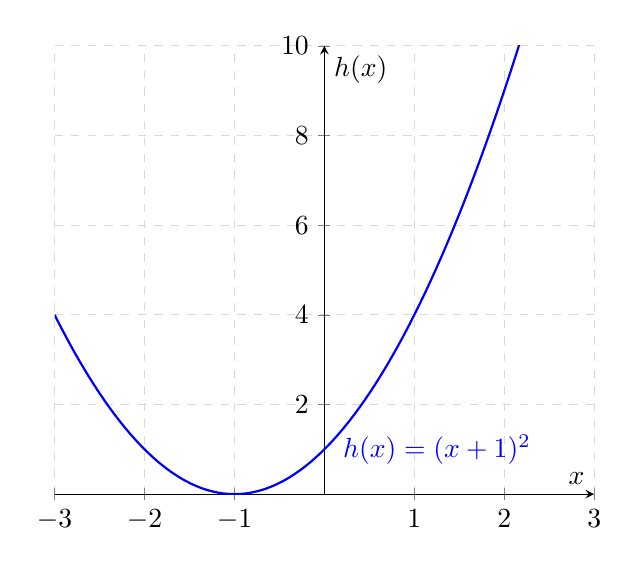
\begin{tikzpicture}
\begin{axis}[
    axis lines=middle,
    xlabel={$x$},
    ylabel={$h(x)$},
    xmin=-3, xmax=3,
    ymin=0, ymax=10,
    xtick={-3,-2,...,3},
    ytick={0,2,...,10},
    grid=major,
    grid style={dashed,gray!30},
]
\addplot[domain=-3:3, samples=100, color=blue, thick] {(x+1)^2};
\node[anchor=west, blue] at (axis cs:0.1,1) {$h(x) = (x+1)^2$};

\end{axis}
\end{tikzpicture}
}
\end{enumerate}\hfill\\
\end{exercise}


\begin{exercise}\label{ex:operationen_funktionen}
Definieren Sie die Funktionen $f+g$, $f-g$, $f\cdot g$ und $\frac{f}{g}.$ Wenn möglich, definieren Sie zudem die Funktionen $f \circ g$ und $g \circ f$ mit einem adäquaten Definitionsbereich.
{\scriptsize
\begin{enumerate}[2col, label=\roman*)]
\item \begin{IEEEeqnarray*}{rCcCLCRCcCl}
  f &: & [0,1] & \rightarrow & \mathbb{R}, &\quad & g &: & [1,2] & \rightarrow & \mathbb{R}\\
  & &x &\mapsto & x^2& &\quad& &t &\mapsto & t+1
\end{IEEEeqnarray*}

\item \begin{IEEEeqnarray*}{rCcCLCRCcCl}
  f &: & \mathbb{R} & \rightarrow & \mathbb{R}, &\quad & g &: & \mathbb{R}_{\geqslant 0} & \rightarrow & \mathbb{R}\\
  & &x &\mapsto & 5x+4& &\quad& &t &\mapsto & 6t+1\\
\end{IEEEeqnarray*}
\item \begin{IEEEeqnarray*}{rCcCLCRCcCl}
  f &: & [0,5] & \rightarrow & \mathbb{R}, &\quad & g &: & ]-1,10] & \rightarrow & \mathbb{R}\\
  & &x &\mapsto & x^2& &\quad& &t &\mapsto & \frac{1}{t+1}
\end{IEEEeqnarray*}

\item \begin{IEEEeqnarray*}{rCcCLCRCcCl}
  f &: & \mathbb{R} & \rightarrow & \mathbb{R}, &\quad & g &: & ]0,10] & \rightarrow & \mathbb{R}\\
  & &x &\mapsto & x^2-1& &\quad& &t &\mapsto & \frac{1}{t}\\
\end{IEEEeqnarray*}
\end{enumerate}%\hfill\\
}
\end{exercise}

%\newpage
%\subsection{Weitere Beispiele}
%%\begin{example}
%Ein gutes Beispiel für eine Funktion ist die Beziehung zwischen der Temperatur in Grad Celsius und in Grad Fahrenheit.
%\begin{example}\label{exmpl:fahrenheit}
%Die Temperatur in Grad Fahrenheit kann als Funktion der Temperatur in Grad Celsius ausgedrückt werden: es sei $f$ die Funktion definiert als:
%\begin{IEEEeqnarray*}{rCcCl}
%  %\subnumberinglabel{eq:1}
%  f &: & \mathbb{R} & \rightarrow & \mathbb{R}\\
%  & &c &\mapsto & \frac{5}{9} c + 32,
%\end{IEEEeqnarray*}
%dann entspricht $f(c)$ der Temperatur in Grad Fahrenheit, wenn $c$ die Temperatur in Grad Celsius ist.
%\end{example}
%
%
%Weitere, etwas abstraktere Beispiele für Funktionen sind etwa die Beziehung zwischen dem Einkommen und der zu zahlenden Einkommenssteuer im Kanton Aargau (siehe Abbildung~\ref{fig:steuer}), die Beziehung zwischen den Buchstaben und ihrer Position im Alphabet (\emph{``A''} entspricht Position 1, \emph{``B''} entspricht Position 2, \emph{``C''} entspricht Position 3 usw., bis \emph{``Z''}), oder auch die Beziehung zwischen dem Alter einer Person und dem heutigen Datum.
%\begin{figure}
%\begin{center}
%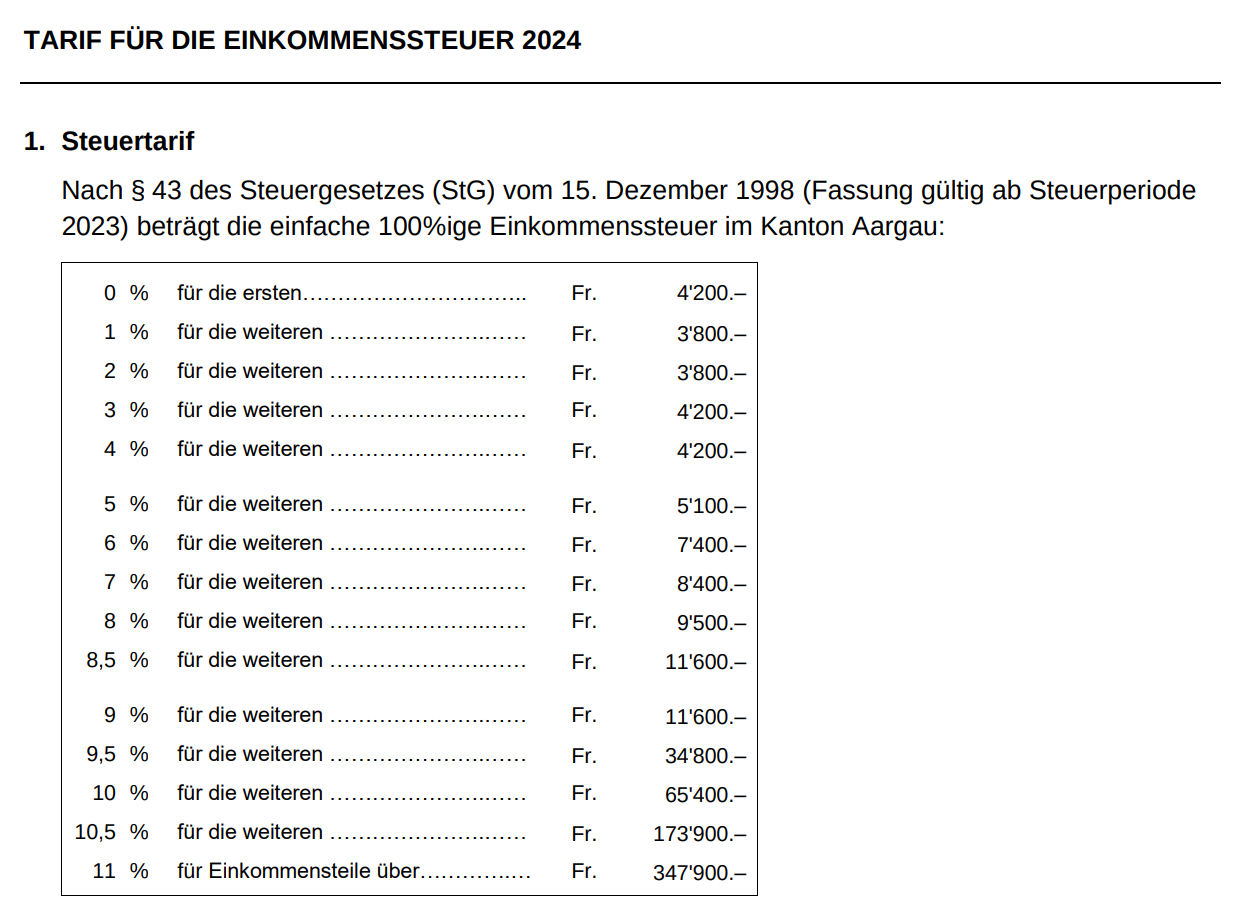
\includegraphics[width=0.9\textwidth]{figures/steuer_aargau.png}
%\end{center}
%\caption{Steuerprogression Kanton Aargau 2024, \href{https://www.ag.ch/media/kanton-aargau/dfr/dokumente/steuern/natuerliche-personen/steuerberechnung-tarife-natuerliche-personen/einkommenssteuertarif-2024.pdf}{https://www.ag.ch/}}\label{fig:steuer} 
%\end{figure}
\newpage
\subsection{Reflexion zum Begriff der Funktion}
Bitte lesen Sie die Lernziele dieses Kapitels auf Seite~\pageref{goals:funktionen_begrifflichkeit} aufmerksam durch. Gibt es Dinge, mit denen Sie sich nochmal auseinandersetzen möchten? Schreiben Sie diese jetzt hier auf. Sie dürfen mir übrigens auch e-mails schreiben, falls Sie Fragen zum Unterrichtsinhalt haben.\\

\begin{tcolorbox}[reflectionbox, width=\linewidth]
\begin{tabularx}{\textwidth}{|X|X|}
\toprule
\textbf{Möchte ich noch vertiefen}\\[6cm]
\bottomrule
\end{tabularx}
\end{tcolorbox}\\
\noindent
Ich würde Sie bitten, sich hier kurz zu notieren, welche Aspekte an diesem Kapitel Ihnen gefallen haben und welche Sie lieber anders erlebt hätten.\\
\begin{tcolorbox}[reflectionbox, width=\linewidth]
\begin{tabularx}{\textwidth}{|X|X|}
\toprule
\textbf{Hat mir gefallen} & \textbf{Hat mir nicht gefallen}\\[5cm]
\bottomrule
\end{tabularx}
\end{tcolorbox}

\newpage
\section{Lineare Funktionen}

Sie dürften mit dem Begriff der linearen Funktion bereits vertraut sein. Der Vollständigkeit wegen wird er hier noch einmal definiert.
\begin{whitebox}
\begin{definition}
Eine Funktion von den reellen Zahlen in die reellen Zahlen heisst \emph{linear}, wenn ihr Graph eine Gerade abbildet.

\noindent
Eine lineare Funktion $f$ mit Funktionsargument $x$ entspricht der folgenden Form
\begin{IEEEeqnarray*}{rCcCl}
  f &: & \mathbb{R} & \rightarrow & \mathbb{R}\\
  & &x &\mapsto & a x + b,
\end{IEEEeqnarray*}
wobei $a$ und $b$ reelle konstanten sind.

Folgende Begriffe werden benutzt, um lineare Funktionen zu charakterisieren:
\begin{itemize}
\item Die \textbf{Steigung} entspricht dem Multiplikator des Funktionsarguments. Im gegebenen Fall also $a$. Manchmal wird $a$ auch \textbf{Steigungskoeffizient} genannt.

%Die Steigung entspricht der \textbf{konstanten Änderungsrate}: wenn das Funktionsargument um eine Einheit wächst, wächst der Funktionswert um $a$ Einheiten. Diese Änderungsrate ist konstant, da sie unabhängig vom Ausgangswert des Funktionsarguments gleich gross ist. Dies ist ein Merkmal von linearen Funktionen.
\item Der \textbf{Ordinatenabschnitt} (oder auch y-Achsenabschnitt), entspricht dem Wert der Funktion mit Argument null. Im gegebenen Fall ist das die Konstante $b$, da $f(0)=b$.

Graphisch entspricht der Ordinatenabschnitt der Höhe, in welcher der Funktionsgraph die vertikale Achse schneidet (siehe Abbildung~\ref{fig:lin_func}).
\item Sofern die {Steigung} nicht gleich Null ist, weist $f$ genau eine \textbf{Nullstelle} auf. Das ist der Punkt $x_0$, in dem der Funktionswert Null ist, also für welchen gilt $f(x_0) = 0.$

Graphisch entspricht der Nullpunkt dem Schnittpunkt des Funktionsgraphen mit der horizontalen Achse (siehe Abbildung~\ref{fig:lin_func}).
\end{itemize}
\end{definition}
\end{whitebox}

%Die \textbf{Steigung} $a$ gibt den konstanten Änderungsfaktor von $f(x)$, pro Einheit in $x$ an: wenn das Funktionsargument um eine Einheit wächst, dann wächst der Funktionswert um $a$:
%\begin{IEEEeqnarray*}{lCl}
%f(x + 1) &=& a(x + 1) + c\\
%&=& a x + a + c\\
%&=& (a x + c) + a\\
%&=& f(x) + a
%\end{IEEEeqnarray*}
\begin{figure}[h]
\begin{center}
\begin{tikzpicture}[>=Stealth, scale=0.8]
    % Draw axes
    \draw[->] (-6,0) -- (6,0) node[right] {$x$};
    \draw[->] (0,-3) -- (0,9) node[above] {$y(x)$};

	 % Draw grid
    \draw[very thin, color=gray!30] (-6,-3) grid (6,9); % Grid lines

    % Add ticks and labels on x-axis
    \foreach \x in {-6,...,6}
        \draw (\x,0.1) -- (\x,-0.1) node[below] {\tiny $\x$};

    % Add ticks and labels on y-axis
    \foreach \y in {-3,...,9}
        \draw (0.1,\y) -- (-0.1,\y) node[left] {\tiny $\y$};

    % Define linear function f(x) = 2x + 1
    \draw[thick, black] (-2,-3) -- (4,9) node[below right] {$y(x)=2x + 1$};

    % Highlight the y-intercept
    \filldraw[blue] (0,1) circle (2pt);
	\draw[decorate, decoration={brace, amplitude=5pt, mirror, raise=1ex}, blue] (0,0) -- (0,1) node[midway, xshift = 6em] {$\textit{Ordinatenabschnitt} = 1$};
	
    % Highlight the zero of the function (x-intercept)
    \draw[decorate, decoration={brace, amplitude=5pt, mirror, raise=1ex}, red] (-0.5,0) -- (0,0) node[midway, yshift = -1.5em, xshift = 3em] {$\textit{Nullstelle} = -0.5$};
    \filldraw[red] (-0.5,0) circle (2pt); %node[above left, red] {\textit{Nullstelle} (-0.5,0)};

    % Draw slope triangle for demonstration
    \draw[thick, orange, dashed] (1,3) -- (3,3) node[below, midway] {$\Delta x$};
    \draw[thick, orange, dashed] (3,3) -- (3,7) node[right, midway] {$\Delta y$};
    \draw[thick, orange, dashed] (3,7) -- (1,3);

    %\draw (0.5,0) -- (0.5,0.1) -- (0.6,0.1); % Small right angle symbol
    \node at (3,3) [below, right, orange] {$\textit{Steigung} = \frac{\Delta y}{\Delta x} = 2$};
\end{tikzpicture}
\caption{Funktionsgraph für $y(x) = 32+1$}\label{fig:lin_func}
\end{center}
\end{figure}


\begin{lemma}\label{lemma:ermittlung_steigung}
Es sei $f : \mathbb{R} \rightarrow \mathbb{R}$ eine lineare Funktion und $x_1, x_2$ zwei reelle Zahlen, so dass $x_1 \neq x_2$. Dann ist die Steigung von $f$ gegeben durch $\frac{f(x_2) - f(x_1)}{x_2-x_1}.$
\end{lemma}
Geometrisch entspricht dieses Ermittlungsverfahren dem Steigungsdreieck (siehe Abbildung~\ref{fig:lin_func}, in orange eingezeichnet).

Wir können die Behauptung auch formell beweisen.

\begin{proof}
Wenn $f$ eine lineare Funktion ist, dann gibt es reelle Koeffizienten $a$ und $b$, so dass $f(x) = ax + b,$ für alle $x \in \mathbb{R}$.

Es seien $x_1, x_2$ zwei unterschiedliche reelle Zahlen. Dann finden wird: 
\begin{IEEEeqnarray*}{lCl}
\frac{f(x_2) - f(x_1)}{x_2-x_1} &=& \frac{(a x_2 + c) - (a x_1+c)}{x_2-x_1}\\
&=& \frac{ax_2 + c - a x_1+c}{x_2-x_1}\\
&=& \frac{ax_2 - a x_1}{x_2-x_1}\\
&=& \frac{a(x_2 - x_1)}{x_2-x_1}\\
&=& a,
\end{IEEEeqnarray*}
somit ist bewiesen, dass $\frac{f(x_2) - f(x_1)}{x_2-x_1}$ dem Steigungskoeffizienten entspricht.
\end{proof}

\begin{remark}
Lemma~\ref{lemma:ermittlung_steigung} impliziert, dass die Steigung $a$ gegeben ist durch $f(x+1)-f(x)$, für jedes beliebige $x \in \mathbb{R}$.
\end{remark}


\begin{exercise}
Es sei $f$ eine lineare Funktion und $(-112, 854), (-12.3, 10)$ zwei Wertepaare der Funktion. Bestimmen Sie den Ordinatenabschnitt, die Steigung und die Nullstelle der Funktion.
\end{exercise}
\subsection{Lineare Funktionen graphisch darstellen}
Lineare Funktionen gehören zu den Funktionen, die sich graphisch am einfachsten darstellen lassen, da sie eine gerade Linie sind.

Man braucht nur zwei Punkte einzeichnen, die auf der Geraden liegen, und dann beide Punkte mit dem Dreieck verbinden.

Einen Punkt, den Ordinatenabschnitt, bekommt man gratis. Den zweiten Punkt kann man ermitteln, indem man die Funktion mit einem geeigneten Argument evaluiert.

\begin{example}
\begin{enumerate}[label=\alph*)]
\item Die lineare Funktion $f: \mathbb{R} \rightarrow \mathbb{R},\; x \mapsto 2x+1$ lässt sich z.B. in folgenden Schritten darstellen:
\begin{enumerate}[label=\arabic*)]
\item Der Ordinatenabschnitt ist $1$, deshalb weiss ich, dass die Gerade durch den Punkt $(0,1)$ verläuft und kann diesen im Koordinatensystem markieren:
\begin{center}
\resizebox{0.5\linewidth}{!}{
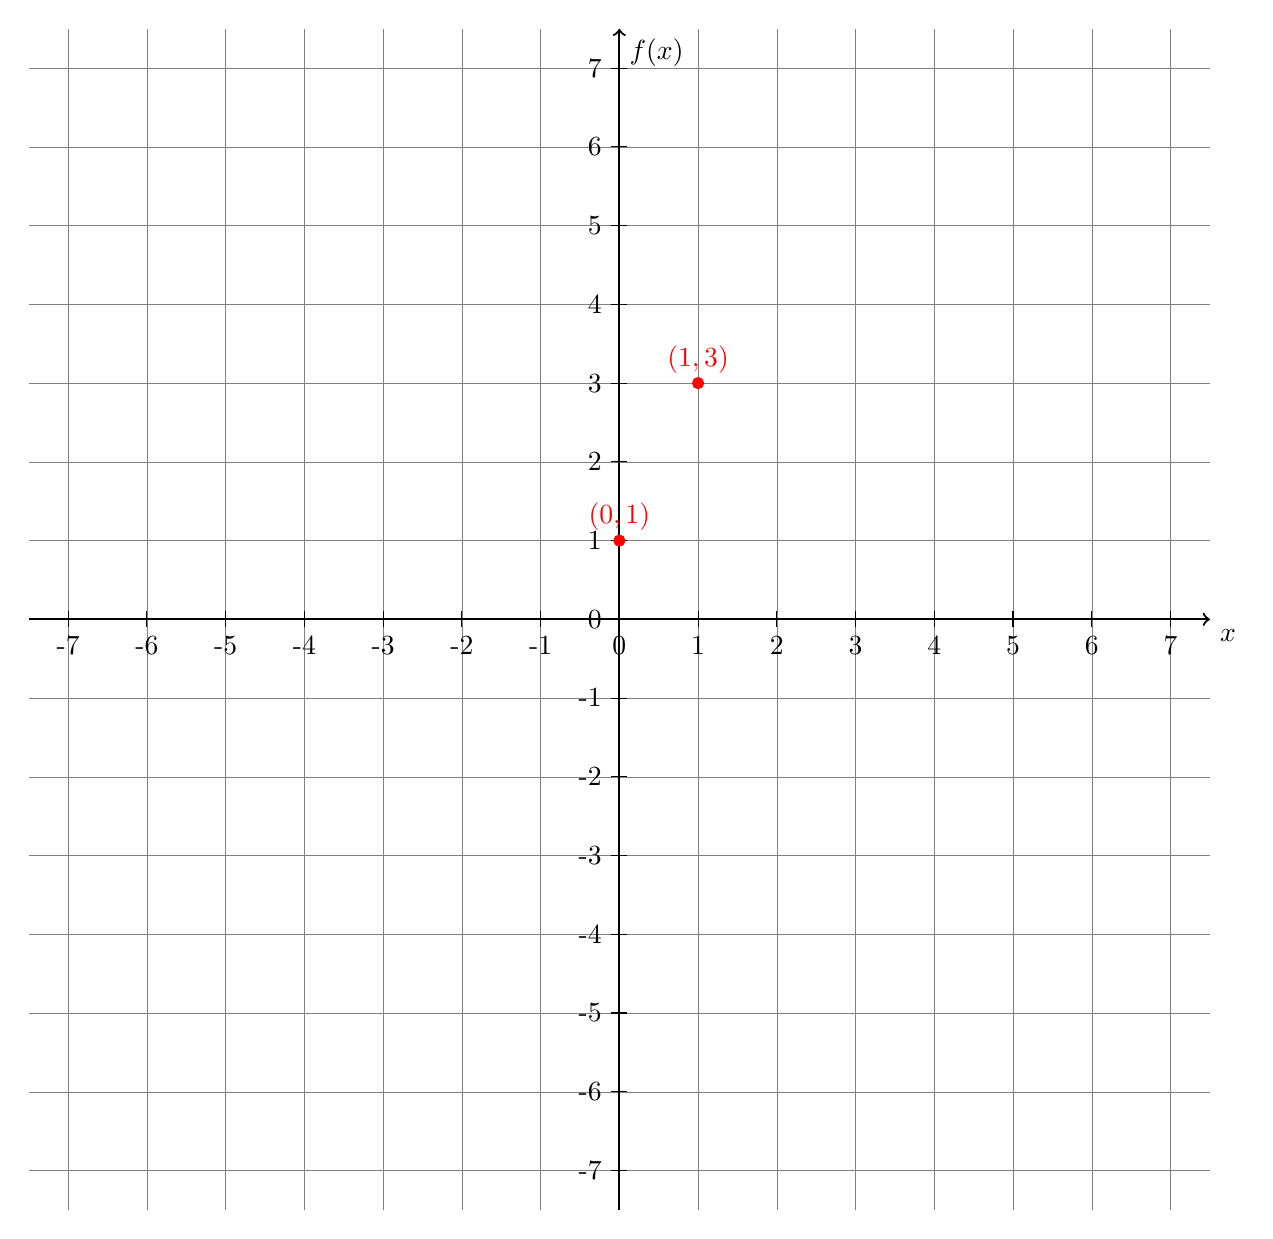
\begin{tikzpicture}
\draw[step=1cm,gray,very thin] (-7.5,-7.5) grid (7.5,7.5);
\draw[thick,->] (-7.5,0) -- (7.5,0) node[anchor=north west] {$x$};
\draw[thick,->] (0,-7.5) -- (0,7.5) node[anchor=north west] {$f(x)$};
\foreach \x in {-7,-6,...,7}
    \draw (\x,0.1) -- (\x,-0.1) node[anchor=north] {\x};
\foreach \y in {-7,-6,...,7}
    \draw (0.1,\y) -- (-0.1,\y) node[anchor=east] {\y};

% Mark the points (0,1) and (1,3)
\filldraw [red] (0,1) circle (2pt) node[anchor=south] {$(0,1)$};
\filldraw [red] (1,3) circle (2pt) node[anchor=south] {$(1,3)$};
\end{tikzpicture}
}
\end{center}
\item Wenn ich die Funktion im Wert $1$ evaluiere, erhalte ich den Funktionswert $f(1)= 2+1 = 3.$ Somit weiss ich, dass der Punkt $(1,3)$ ebenfalls auf der Geraden liegt. Diesen Punkt kann ich nun ebenfalls im Koordinatensystem einzeichnen
\begin{center}
\resizebox{0.5\linewidth}{!}{
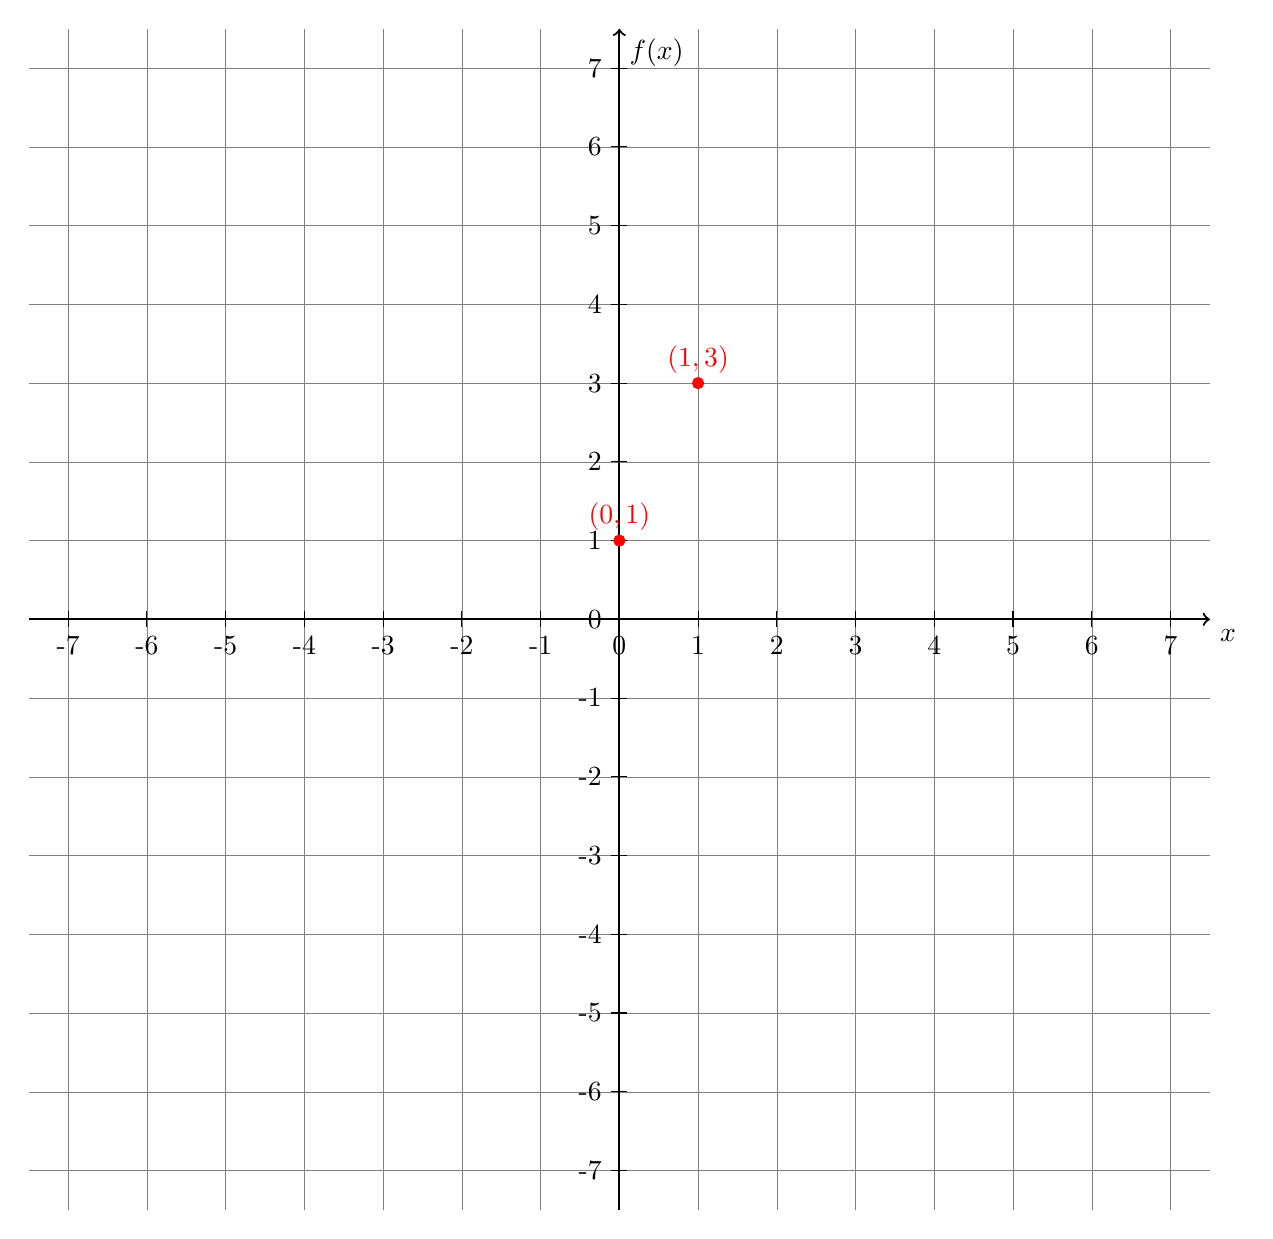
\begin{tikzpicture}
\draw[step=1cm,gray,very thin] (-7.5,-7.5) grid (7.5,7.5);
\draw[thick,->] (-7.5,0) -- (7.5,0) node[anchor=north west] {$x$};
\draw[thick,->] (0,-7.5) -- (0,7.5) node[anchor=north west] {$f(x)$};
\foreach \x in {-7,-6,...,7}
    \draw (\x,0.1) -- (\x,-0.1) node[anchor=north] {\x};
\foreach \y in {-7,-6,...,7}
    \draw (0.1,\y) -- (-0.1,\y) node[anchor=east] {\y};

% Mark the points (0,1) and (1,3)
\filldraw [red] (0,1) circle (2pt) node[anchor=south] {$(0,1)$};
\filldraw [red] (1,3) circle (2pt) node[anchor=south] {$(1,3)$};
\end{tikzpicture}
}
\end{center}
\item anschliessend lassen sich beide Punkte durch eine gerade Linie verbinden:
\begin{center}
\resizebox{0.5\linewidth}{!}{
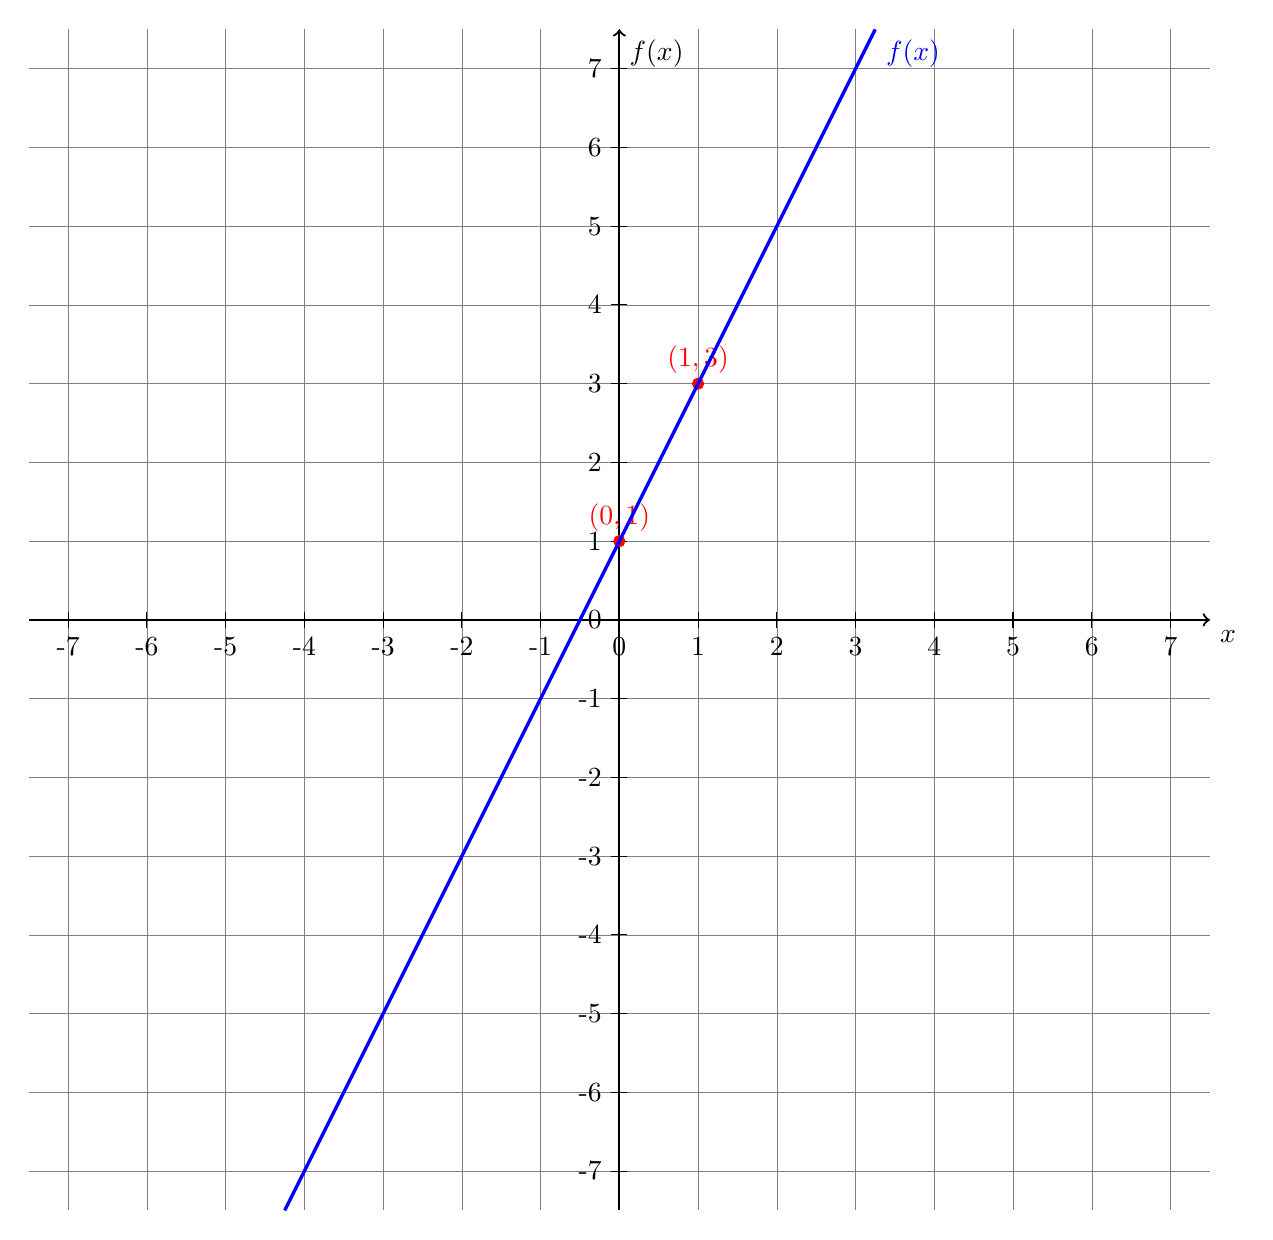
\begin{tikzpicture}
\draw[step=1cm,gray,very thin] (-7.5,-7.5) grid (7.5,7.5);
\draw[thick,->] (-7.5,0) -- (7.5,0) node[anchor=north west] {$x$};
\draw[thick,->] (0,-7.5) -- (0,7.5) node[anchor=north west] {$f(x)$};
\foreach \x in {-7,-6,...,7}
    \draw (\x,0.1) -- (\x,-0.1) node[anchor=north] {\x};
\foreach \y in {-7,-6,...,7}
    \draw (0.1,\y) -- (-0.1,\y) node[anchor=east] {\y};

% Mark the points (0,1) and (1,3)
\filldraw [red] (0,1) circle (2pt) node[anchor=south] {$(0,1)$};
\filldraw [red] (1,3) circle (2pt) node[anchor=south] {$(1,3)$};
\draw[very thick, blue] (-4.25,-7.5) -- (3.25,7.5) node[anchor=north west] {$f(x)$}; % Extended line for visibility
\end{tikzpicture}
}
\end{center}
\end{enumerate}
\end{enumerate}
\end{example}

\begin{remark}
Manchmal sind der Steigungskoeffizient oder der Ordinatenabschnitt keine ganzen Zahlen. In einem solchen Fall ergibt obige Strategie auch keine Punkte, die auf dem Koordinatenraster liegen. Dann muss ich entweder mit dem Geodreick oder Masstab messen, oder aber, ich versuche andere Punkte zu finden, die auf der Gerade und dem Raster liegen.
\end{remark}
\subsection{Übungen}
\begin{exercise}
\begin{enumerate}[label=\alph*)]
\item Es sei $f$ eine lineare Funktion, zu der zwei Wertepaare $(0,5)$ und $(1,-2)$ gehören. Bestimmen Sie: \begin{enumerate}[label=\roman*)]
\item die Steigung der Funktion;
\item den Ordinatenabschnitt der Funktion;
\item den Nullpunkt der Funktion.
\end{enumerate}
Definieren Sie die Funktion formal.
\item Es seien $f, g$ und $h$ drei lineare Funktionen, wie im Graphen abgebildet.
\begin{enumerate}[label=\roman*)]
\item Definieren Sie die Funktionen $f, g$ und $h$ mathematisch;
\item Bestimmen Sie den Schnittpunkt von $f$ und $g$;
\end{enumerate}
\begin{center}
\begin{tikzpicture}[>=Stealth, scale=0.6]
    % Draw axes
    \draw[->] (-6,0) -- (6,0) node[right] {$x$};
    \draw[->] (0,-3) -- (0,9) node[above] {$y$};

	 % Draw grid
    \draw[very thin, color=gray!30] (-6,-3) grid (6,9); % Grid lines

    % Add ticks and labels on x-axis
    \foreach \x in {-6,...,6}
        \draw (\x,0.1) -- (\x,-0.1) node[below] {\tiny $\x$};

    % Add ticks and labels on y-axis
    \foreach \y in {-3,...,9}
        \draw (0.1,\y) -- (-0.1,\y) node[left] {\tiny $\y$};

    % Define linear function f(x) = -5x + 3
    \draw[thick, blue] (1.2,-3) -- (-1.2,9)  node[left] {$y = f(x)$};
    % Define linear function f(x) = -5x + 3
    \draw[thick, red] (2,-3) -- (6,9) node[below right] {$y = g(x)$};
    \draw[thick, orange] (-6,1) -- (6, 1) node[above right] {$y = h(x)$};
\end{tikzpicture}
\end{center}
\item In Aufgabe~\ref{ex:temp_fahrenheit} wird erklärt, wie man Grad Celsius in Grad Fahrenheit umrechnen kann. Bestimmen Sie die inverse Funktion, also die Funktion, die Grad Fahrenheit in Grad Celsius umrechnet. Was ist der Ordinatenabschnitt, was ist die Steigung, wo ist der Nullpunkt? Zeichnen Sie den Graphen der Funktion.
\begin{center}
\begin{tikzpicture}[>=Stealth, scale=0.5]
    % Draw axes
    %\draw[->] (-6,0) -- (6,0) node[right] {$x$};
    %\draw[->] (0,-3) -- (0,9) node[above] {$y$};

	 % Draw grid
    \draw[very thin, color=gray!30] (-10,-10) grid (10,10); % Grid lines

    % Add ticks and labels on x-axis
    %\foreach \x in {-6,...,6}
    %    \draw (\x,0.1) -- (\x,-0.1) node[below] {\tiny $\x$};

    % Add ticks and labels on y-axis
    %\foreach \y in {-3,...,9}
    %    \draw (0.1,\y) -- (-0.1,\y) node[left] {\tiny $\y$};

    % Define linear function f(x) = -5x + 3
    %\draw[thick, blue] (-1.2,9) -- (1.2,-3) node[below right] {$f(x)$};
    % Define linear function f(x) = -5x + 3
    %\draw[thick, red] (2,-3) -- (6,9) node[below right] {$g(x)$};
    %\draw[thick, orange] (-6,1) -- (6, 1) node[below right] {$h(x)$};
\end{tikzpicture}
\end{center}
\end{enumerate}
\end{exercise}


\newpage
\section{Quadratische Funktionen}

\begin{exercise}\label{ex:konfrontation_quadratische_funktion}
Es seien folgende Funktionen gegeben:
\begin{IEEEeqnarray*}{rCrClCrCrCl}
f &:& \Reals & \rightarrow & \Reals
& \quad &
w &:& \Reals & \rightarrow & \Reals\\
&& x & \mapsto & x^2 && 
&& x & \mapsto & x^2 + 5x + 2\\
h &:& \Reals & \rightarrow & \Reals
& \quad &
u &:& \Reals & \rightarrow & \Reals\\
&& x & \mapsto & -x^2 + x + 10 &&
&& x & \mapsto & 2x^2 + 3
\end{IEEEeqnarray*}
\begin{enumerate}[label=\alph*)]
\item Bestimmen Sie den Ordinatenabschnitt für jede der Funktionen (das ist der Funktionswert im Punkt Null. Das ist auch die Distanz zwischen dem Ursprung und dem Schnittpunkt vom Funktionsgraphen mit der vertikalen Achse).

\item Bestimmen Sie, welcher der Funktionsgraphen in unterer Abbildung jeweils zu $f$, $h, w$ und $u$ gehört. Begründen Sie Ihre Aussage.
\begin{center}

\resizebox{0.8\linewidth}{!}{
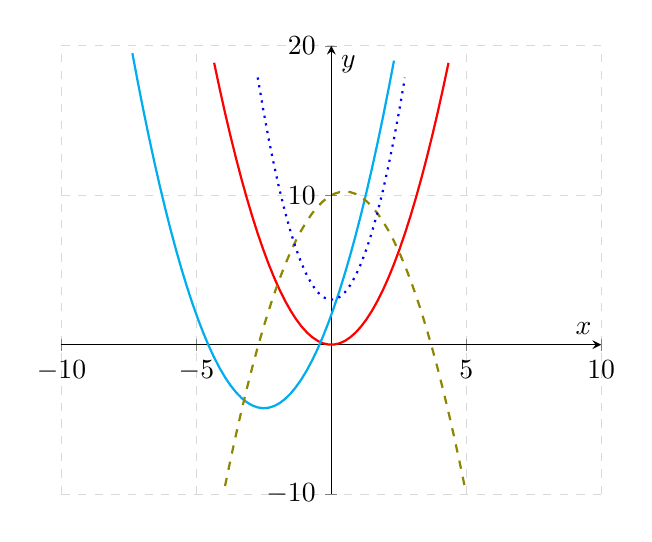
\begin{tikzpicture}
\begin{axis}[
    axis lines=middle,
    xlabel={$x$},
    ylabel={$y$},
    xmin=-10, xmax=10,
    ymin=-10, ymax=20,
    restrict y to domain=-10:20,
    %legend pos=north west,
    %legend style={draw=none},
    clip=false,
    grid=major,
    grid style={dashed,gray!30}
]

% Function f(x) = x^2
\addplot[domain=-10:10, samples=100, red, thick] {x^2};
%\addlegendentry{$f(x) = x^2$}

% Function w(x) = x^2 + 5x + 2
\addplot[domain=-10:10, samples=100, cyan, thick] {x^2 + 5*x + 2};
%\addlegendentry{$w(x) = x^2 + 5x + 2$}

% Function h(x) = -x^2 + x + 10
\addplot[domain=-10:10, samples=100, olive, thick, dashed] {-x^2 + x + 10};
%\addlegendentry{$h(x) = -x^2 + x + 10$}

% Function u(x) = -x^2 + x + 10
\addplot[domain=-10:10, samples=100, blue, thick, dotted] {2*x^2 + 3};
%\addlegendentry{$h(x) = -x^2 + x + 10$}
\end{axis}
\end{tikzpicture}
}
\end{center}

%\item Man nennt einen Punkt $x_0 \in \Reals$ eine Nullstelle einer Funktion $g : \mathbb{R} \rightarrow \Reals$, wenn $f(x_0)=0$ gilt. Bestimmen Sie für jede der Funktionen die Anzahl Nullstellen, die sie hat.
\item Aufgrund des Funktionsgraphen, äussern Sie eine Vermutung zu jeder Funktion, ob diese nach oben oder unten begrenzt ist, das heisst, ob der Funktionswert zwingend kleiner, respektive grösser, als ein gewisser Wert sein muss. Können Sie ihre Vermutung mathematisch begründen? Was passiert mit dem Funktionswert, wenn das Funktionsargument gegen $+\infty$ oder gegen $-\infty$ strebt?
\item Welche Funktionen vermuten Sie als injektiv? Welche glauben Sie, sind surjektiv?
\end{enumerate}
\end{exercise}


\subsection{Allgemeine Form}
Funktionen wie in Aufgabe~\ref{ex:konfrontation_quadratische_funktion} werden als \textbf{quadratische Funktionen} bezeichnet. Ihr Funktionsgraph ist ein ist einem ``u'' oder einem auf den Kopf gedrehten ``u'' ähnlich. Quadratische Funktionen sind dadurch erkennbar, dass sie das Funktionsargument quadrieren.


\begin{whiteboxdef}
Es seien $A$ und $B$ zwei Teilmengen der reellen Zahlen.

Eine Funktion $f : A \rightarrow B$ heisst \textbf{quadratische Funktion}, wenn drei reelle Konstanten $a,b,c \in \mathbb{R}$ existieren, so dass $a \neq 0$ und so dass gilt:
\begin{IEEEeqnarray}{rClCr}\label{eq:allgemeine_form_quad_func}
f(x) &=& ax^2 + bx + c, &\quad &\forall \; x \in A.
\end{IEEEeqnarray}

Diese Schreibweise für quadratische Funktionen heisst \textbf{allgemeine Form}.
\end{whiteboxdef}
\begin{remark}
Eine Menge $S$ ist eine \textbf{Teilmenge} der Menge $M$, wenn jedes Element in $S$ auch ein Element in $M$ ist (\emph{$S$ ist \emph{``ein Teil''} aus $M$}. Symbolisch lässt sich das als ``$S \subseteq M$'' abkürzen).

Zum Beispiel ist die Menge der nicht-positiven reellen Zahlen $\mathbb{R}_{\leqslant 0}$ eine Teilmenge der reellen Zahlen. Eine Menge ist immer auch eine Teilmenge seiner selbst (z.B. ist $\mathbb{R}$ eine Teilmenge von $\mathbb{R}$, nämlich \emph{``der ganze Teil''} von $\mathbb{R}$).


Das Symbol $\forall$ bedeutet \textbf{\emph{``für alle''} oder \emph{``für jedes''}}. Gleichung~\ref{eq:allgemeine_form_quad_func} lässt sich also wie folgt aussprechen:
\emph{Der Funktionswert von $f$ im Punkt $x$ ist gleich dem Wert des Terms $ax^2 + bx + c$, und zwar für jedes Element $x$ aus der Definitionsmenge $A$}.
\end{remark}
\begin{example}
\begin{enumerate}[label=\alph*)]
\item Funktion A aus Beispiel~\ref{ex:square}, welche die Seitenlänge eines Quadrates seiner Fläche zuordnet, ist eine quadratische Funktion. Hier ist nochmals ihre Definition:
\begin{IEEEeqnarray*}{rCrCl}
A &:& \mathbb{R}_{\geqslant 0} &\rightarrow &\mathbb{R}\\
&& l &\mapsto & l^2.
\end{IEEEeqnarray*}
Die Funktion $A$ ist quadratisch, weil Gleichung~\ref{eq:allgemeine_form_quad_func} für $a=1, b=0$ und $c=0$ hält. Wir finden nämlich, für jedes $x \in \mathbb{R}_{\geqslant 0}$:
\begin{IEEEeqnarray*}{rCl}
A(x) &=& x^2\\
&=& a x^2 + 0 \cdot x + 0
\end{IEEEeqnarray*}
\item Die Funktion $v$, wie folgt definiert, ist quadratisch:
\begin{IEEEeqnarray*}{rCrCl}
v &:& \mathbb{R}_{\geqslant 0} &\rightarrow &\mathbb{R}\\
&& t &\mapsto & 5t^2 + 6t + 10,
\end{IEEEeqnarray*}
da Geichung~\ref{eq:allgemeine_form_quad_func} erfüllt wird mit $a=5, b=6$ und $c=10$.
\item Es seien $g$ und $h$ reelle lineare Funktionen, wie folgt definiert:
\begin{IEEEeqnarray*}{rCrClCrCrCl}
g & : & \Reals &\rightarrow &\Reals & \quad & h & : & \Reals &\rightarrow & \Reals\\
&& x &\mapsto & 4x+1 & & & & y &\mapsto & -6y+10,
\end{IEEEeqnarray*}
Das Produkt der Funktionen $g$ und $h$ ist wiederum eine Funktion, $f = g \cdot h$, die wie folgt definiert ist:
\begin{IEEEeqnarray*}{rCrCl}
f &: & \Reals & \rightarrow &\Reals\\
&& x &\mapsto & g(x) \cdot h(x).
\end{IEEEeqnarray*}
Die Funktion $f$ ist eine quadratische Funktion, denn es gilt für jedes $x \in \mathbb{R}:$
\begin{IEEEeqnarray*}{rCl}
f(x) &=&  g(x) \cdot h(x)\\
&=& (4x+1)(-6x+10)\\
&=& 4x\cdot (-6x+10) + 1\cdot (-6x+10)\\
&=& -24x^2 + 40x -6x +10\\
&=& -24x^2 +34x + 10,
\end{IEEEeqnarray*}
somit ist Gleichung~\ref{eq:allgemeine_form_quad_func} für $a=-24, b=34$ und $c=10$ erfüllt.
\end{enumerate}
\end{example}

\begin{exercise}\label{ex:quad_func_allgemein_params}
Es seien $f, h, w$ und $u$ wie aus Aufgabe~\ref{ex:konfrontation_quadratische_funktion}. Bestimmen Sie für jede der Funktionen die Parameter $a,b,c,$ so dass ihre Zuordnung als $ax^2 + bx + c$ geschrieben werden kann.
\end{exercise}

\begin{exercise}\label{ex:quad_func_allgemein_einfluss_params}
Greifen Sie auf das vorbereitete Geogebra Arbeitsblatt zu und verbringen Sie einige Minuten damit, ein Gefühl für die Parameter $a,b$ und $c$ zu erhalten.
\begin{itemize}
\item Welchen Parameter müssen Sie ändern, wenn Sie den Funktionsgraphen vertikal nach oben oder unten verschieben möchten?
\item Welche Rolle spielt das Vorzeichen von $a$ für die Form des Funktionsgraphen?
\end{itemize}
\end{exercise}
\begin{remark}
Eine quadratische Funktion $f: \mathbb{R} \rightarrow \mathbb{R},$ ausgedrückt in der allgemeinen Form wie in Gleichung~\ref{eq:allgemeine_form_quad_func}, hat ihren Ordinatenabschnitt immer in $c,$ denn es gilt: $f(0) = c$. (Der Ordinatenabschnitt einer Funktion ist der Funktionswert im Punkt $0$.)

Das Vorzeichen des Parameters $a$ informiert über die Öffnung der Funktion: ist dieser positiv, so ist die Funktion nach oben geöffnet, ist dieser negativ, so ist die Funktion nach unten geöffnet. Dieser Sachverhalt wird in den nächsten Unterkapiteln noch formell bewiesen.
\end{remark}

\begin{exercise}\label{ex:quad_func_allgemein_einfluss_param_c}
Es sei $f: \Reals \rightarrow \Reals, \; f(x) = -x^2 + 2x + 1$.
\begin{enumerate}
\item Verändern Sie die Funktion, so dass sich der Funktionsgraph um $4$ Einheiten nach oben verschiebt.
\item Verändern Sie die Funktion, so dass sich der Funktionsgraph um $2$ Einheiten nach unten verschiebt.
\end{enumerate}
\end{exercise}
%\begin{proposition}
%Es sei $f$ eine quadratische Funktion mit Definitionsmenge und Zielmenge $\Reals$ und Parameter $a,b,c$, also so dass
%
%\begin{IEEEeqnarray*}{rCrCl}
%f & \Reals &\rightarrow & \Reals\\
%&& x &\mapsto & ax^2 + bx + c
%\end{IEEEeqnarray*}
%Dann gilt folgendes:
%\begin{enumerate}
%\item Wenn $a > 0$, dann hat die Funktion keinen Maximalwert.
%\item Wenn $a < 0$, dann hat die Funktion keinen Minimalwert.
%\end{enumerate}
%\end{proposition}
\newpage

\subsection{Scheitelpunktform}
\begin{exercise}\label{ex:konfrontation_quadratische_funktion_scheitelpunkt}
\footnotesize
Es seien folgende Funktionen gegeben:
{\footnotesize
\begin{IEEEeqnarray*}{rCrClCrCrCl}
f &:& \Reals & \rightarrow & \Reals
& \quad &
w &:& \Reals & \rightarrow & \Reals\\
&& x & \mapsto & x^2 && 
&& x & \mapsto & (x-1)^2 + 3\\
h &:& \Reals & \rightarrow & \Reals
& \quad &
u &:& \Reals & \rightarrow & \Reals\\
&& x & \mapsto & -(x+2)^2 - 5 &&
&& x & \mapsto & 2x^2 + 3
\end{IEEEeqnarray*}
}
\begin{enumerate}[label=\alph*)]
\item Sind das quadratische Funktionen? Weshalb? Falls ja, bestimmen Sie die allgemeine Form der Funktionen.
\item Bestimmen Sie für jede Funktion den Minimal und Maximalwert, den diese Funktion annehmen kann. Begründen Sie.
\begin{center}
\footnotesize
\begin{tabularx}{\linewidth}{|l|X|X|}
\toprule
Funktion & \makecell{ Funktionsargument \\  \& Minimalwert} & \makecell{  Funktionsargument \\  \& Maximalwert} \\
\midrule
$f(x) = x^2$ & & \\
 & &\\
\hline
$w(x) = (x-1)^2 + 3$ & & \\
 & &\\
\hline
$h(x) = -(x+2)^2 - 5$ &  &\\
& &\\
\hline
$u(x) = 2x^2 + 3$ &  &\\
 & &\\
\bottomrule
\end{tabularx}
\end{center}
\item Bestimmen Sie, welcher der Funktionsgraphen in unterer Abbildung jeweils zu $f$, $h$ und $w$ und $u$ gehört. Begründen Sie Ihre Aussage.
\begin{center}

\resizebox{0.5\linewidth}{!}{
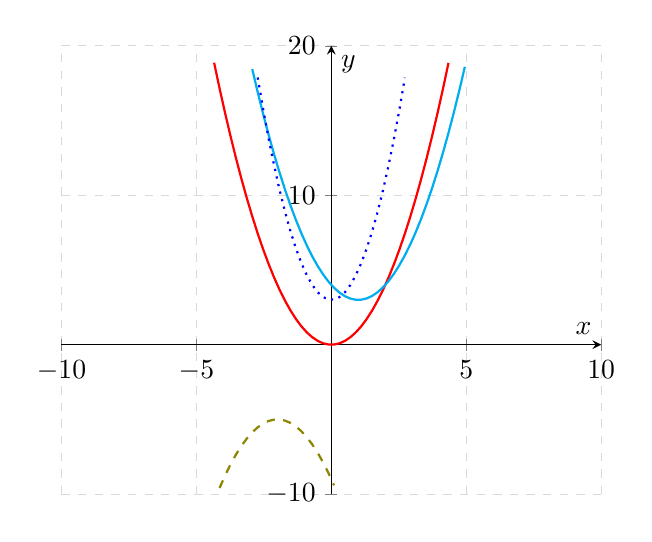
\begin{tikzpicture}
\begin{axis}[
    axis lines=middle,
    xlabel={$x$},
    ylabel={$y$},
    xmin=-10, xmax=10,
    ymin=-10, ymax=20,
    restrict y to domain=-10:20,
    %legend pos=north west,
    %legend style={draw=none},
    clip=false,
    grid=major,
    grid style={dashed,gray!30}
]

% Function f(x) = x^2
\addplot[domain=-10:10, samples=100, red, thick] {x^2};
%\addlegendentry{$f(x) = x^2$}

% Function w(x) = x^2 + 5x + 2
\addplot[domain=-10:10, samples=100, cyan, thick] {(x-1)^2 + 3};
%\addlegendentry{$w(x) = x^2 + 5x + 2$}

% Function h(x) = -x^2 + x + 10
\addplot[domain=-10:10, samples=100, olive, thick, dashed] {-(x+2)^2 - 5};
%\addlegendentry{$h(x) = -x^2 + x + 10$}

% Function u(x) = -x^2 + x + 10
\addplot[domain=-10:10, samples=100, blue, thick, dotted] {2*x^2 + 3};
%\addlegendentry{$h(x) = -x^2 + x + 10$}
\end{axis}
\end{tikzpicture}
}
\end{center}

\end{enumerate}
\end{exercise}

\begin{whiteboxdef}
Es seien $A$ und $B$ zwei Teilmengen der reellen Zahlen und $f: A \rightarrow B$ eine quadratische Funktion, so dass zwei reelle Konstanten $d$ und $e$ existieren und so dass gilt:
\begin{IEEEeqnarray}{rClCl}\label{eq:scheitelpunktform_quad_func}
f(x) &= & a(x-d)^2 + e, &\quad& \forall \; x \in A.
\end{IEEEeqnarray}
Diese Schreibweise für quadratische Funktionen heisst \textbf{Scheitelpunktform}.
\end{whiteboxdef}



\begin{exercise}\label{ex:scheitelpunkt_lueckentext}
Greifen Sie auf das vorbereitete Geogebra Arbeitsblatt zu, um ein Gefühl für die Rolle der Parameter $a, d$ und $e$ aus Gleichung~\ref{eq:scheitelpunktform_quad_func} zu bekommen.
\begin{enumerate}
\item Vervollständigen Sie folgende Sätze:
\begin{itemize}
\setstretch{2.0}
\item Wenn ich den Funktionsgraphen vertikal nach oben verschieben möchte, \rule{3cm}{0.5pt} den Parameter \rule{0.5cm}{0.5pt}
\item  Wenn ich den Funktionsgraphen vertikal nach unten verschieben möchte, \rule{3cm}{0.5pt} den Parameter \rule{0.5cm}{0.5pt}
\item  Wenn ich den Funktionsgraphen horizontal nach rechts verschieben möchte, \rule{3cm}{0.5pt} den Parameter \rule{0.5cm}{0.5pt}
\item  Wenn ich den Funktionsgraphen horizontal nach links verschieben möchte, \rule{3cm}{0.5pt} den Parameter \rule{0.5cm}{0.5pt}
\end{itemize}
\item Auf dem Graphen steht ein Punkt mit \textbf{Scheitelpunkt} angeschrieben. Was sind die Koordinaten dieses Punktes? Man nennt den zugehörigen Funktionswert auch \textbf{Extremwert}, können Sie sich erklären, weshalb er so genannt wird?
\end{enumerate}
\end{exercise}

Wir werden im Kapitel~\ref{subsec:qudratische_ergaenzung} sehen, dass jede quadratische Funktion in der Scheitelpunktform geschrieben werden kann. Gegenüber der allgemeinen Form bietet diese Vorteil, dass der Scheitelpunkt hervorgehoben wird und einfach erkennbar ist. Sie lässt ausserdem erkennen, dass der Funktionsgraph einer quadratischen Funktion eine \textbf{Symmetrieachse} erlaubt, die durch den Scheitelpunkt verläuft. Diesen Umstand werden wir in Satz~\ref{satz:eigenschaften_quad_func} noch formal beweisen.

\begin{figure}[h]
\begin{center}
\begin{tikzpicture}[>=Stealth, scale=0.8]
    % Draw axes
    \draw[->] (-6,0) -- (6,0) node[right] {$x$};
    \draw[->] (0,-3) -- (0,7.5) node[above] {$f(x)$};

	 % Draw grid
    \draw[very thin, color=gray!30] (-6,-3) grid (6,7.5); % Grid lines

    % Add ticks and labels on x-axis
    \foreach \x in {-6,...,6}
        \draw (\x,0.1) -- (\x,-0.1) node[below] {\tiny $\x$};

    % Add ticks and labels on y-axis
    \foreach \y in {-3,...,7}
        \draw (0.1,\y) -- (-0.1,\y) node[left] {\tiny $\y$};

    % Define quadratic function f(x) = 2(x-1) + 3
        \draw[domain=-0.5:2.5, smooth, variable=\x, olive] plot ({\x}, {2*(\x-1)*(\x-1) + 3});
    \node[olive, below right] at (2,4) {$f(x) = 2(x-{\color{blue}{1}})^2 + {\color{red}{3}}$};
    %\draw[thick, black] (-2,-3) -- (4,9) node[below right] {$y(x)=2x + 1$};

    % Highlight the y-intercept
    %\filldraw[blue] (0,1) circle (2pt);
	\draw[decorate, decoration={brace, amplitude=5pt, mirror, raise=1ex}, blue] (0,0) -- (1,0) node[midway, yshift = -2em] {$d=1$};
	
    % Highlight the zero of the function (x-intercept)
    \draw[decorate, decoration={brace, amplitude=5pt, mirror, raise=1ex}, red] (1,0) -- (1,3) node[midway, xshift = 3em] {$e=3$};
    \filldraw[black] (1,3) circle (2pt) node[below left, black] {\textit{Scheitelpunkt}};
    ntercept)
    \draw[magenta, dash dot ] (1,2) -- (1,7.5) node[pos=1, right] {Symmetrieachse für $f(x)$};

    % Draw slope triangle for demonstration
    %\draw[thick, orange, dashed] (1,3) -- (3,3) node[below, midway] {$\Delta x$};
    %\draw[thick, orange, dashed] (3,3) -- (3,7) node[right, midway] {$\Delta y$};
    %\draw[thick, orange, dashed] (3,7) -- (1,3);

    %\draw (0.5,0) -- (0.5,0.1) -- (0.6,0.1); % Small right angle symbol
    %\node at (3,3) [below, right, orange] {$\textit{Steigung} = \frac{\Delta y}{\Delta x} = 2$};
\end{tikzpicture}
\caption{Funktionsgraph für $f(x) = 2(x-1)^2 + 3$ mit Scheitelpunkt $(1,3)$.}\label{fig:scheitelpunkt}
\end{center}
\end{figure}
\begin{proposition}\label{satz:eigenschaften_quad_func}
Eine quadratische Funktion $f: \mathbb{R} \rightarrow \mathbb{R}$ in Scheitelpunktform mit Parametern $a, d$ und $e$, so dass $f(x) = a(x-d)^2 + e, \; \forall \; x \in A,$ erfüllt folgende Eigenschaften:
\begin{enumerate}
\item Wenn $a > 0,$ dann erreicht die Funktion im Punkt $d$ ihr \textbf{Minimum} und nimmt dort den Funktionswert $e$ an.
\item Wenn $a < 0$, dann erreicht die Funktion im Punkt $d$ ihr \textbf{Maximum} und nimmt dort den Funktionswert $e$ an.
\item Es gilt $f(d+x) = f(d-x)$, für alle $x\in \mathbb{R}$.
\emph{Das bedeutet, dass der Funktionsgraph von $f$ um die vertikale Achse, die durch den Punkt $d$ verläuft, symmetrisch ist. Man nennt diese Achse auch \textbf{Symmetrieachse}.}
\end{enumerate}
\end{proposition}
\begin{proof}%
\textbf{Aussage 1:}
Da wir mit den reellen Zahlen arbeiten, ist der Term $(x-d)^2$ für jedes $x \neq d$ positiv, also grösser als Null Wir wissen deshalb, dass der Term $a(x-d)^2$ grösser als Null sein muss, wenn $a >0$ und $x \neq d$ gilt. Deshalb finden wir, dass gilt:
\begin{IEEEeqnarray*}{rCl}
f(x) &=& a(x-d)^2 + e > e.
\end{IEEEeqnarray*}
Entsprechend wissen wir, dass der Funktionswert von $f$ für jedes $x \neq d$ strikt grösser als $e$ sein muss, dass also $f(x) > e,\; \forall x \neq d$ gilt.
Wir finden ausserdem, dass der Funktionswert von $f$ im Punkt $d$ genau $e$ ist, denn es gilt:
\begin{IEEEeqnarray}{rCl}\label{eq:scheitlpunkt_eval_in_d}
f(d) = a(d-d)^2 + e = a \cdot 0^2 + e = e.
\end{IEEEeqnarray}
Wir schlussfolgern dass $f(x) \geqslant e$, für jedes $x \in \Reals,$ womit Aussage 1 beweisen ist. 
\paragraph{Aussage 2:}
Für den Fall dass $a$ negativ ist, dreht sich das Vorzeichen in den obigen Gleichungen um. Wir wissen dann, dass der Funktionswert von $f$ für $x\neq d$ strikt kleiner als $e$ ist. Wir sehen, dass Gleichung~\ref{eq:scheitlpunkt_eval_in_d} auch für negative $a$ gültig ist und können deshalb schlussfolgern, dass wenn $a$ negativ ist, $f(x) \leqslant e, \forall x \in \Reals$ gilt, womit Aussage 2 beweisen ist.

\paragraph{Aussage 3:}
Wir sehen, dass gilt:
\begin{IEEEeqnarray*}{rCl}
f(d+x) &=& a((d+x)-d)^2 +e\\
&=& a(x)^2 + e\\
&=& a (-x)^2 + e\\
&=& a(-x+d-d) + e\\
&=& a((d-x) - d) + e\\
&=& f(d-x),
\end{IEEEeqnarray*}
womit Aussage 3 bewiesen ist.
\end{proof}

%
%\begin{proposition}\label{satz:scheitelpunkt_zu_allgemeine_form}
%Es sei $f: \Reals \rightarrow \Reals$ eine quadratische Funktion in Scheitelpunktform mit Parameter $a, d$ und $e$:
%\begin{IEEEeqnarray*}{rClCl}
%f(x) &= & a(x-d)^2 + e, &\quad& \forall \; x \in A.
%\end{IEEEeqnarray*}
%Dann lässt sich $f$ in allgemeine Form schreiben, mit Parameter $b=-2ad$ und $c=ad^2+e$
%\end{proposition}
%
%\begin{proof}
%Man muss den Zuordnungsterm nur ausmultiplizieren:
%\begin{IEEEeqnarray*}{rCl}
%f(x) &=& a(x-d)^2 + e\\
%&=& a (x^2 - 2xd + d^2) + e\\
%&=&ax^2 \underbrace{\color{orange}-2ad}_{\color{orange}b} x + \underbrace{\color{magenta}ad^2 + e}_{\color{magenta}c},
%\end{IEEEeqnarray*}
%Offensichtlich gilt für $b=-2ad$ und $c=ad^2 + d$, dass der Funktionswert von $f$ in $x$ gleich $ax^2 + bx + c$ ist. Und zwar für jede reelle Zahl $x$.
%\end{proof}


\subsection{Quadratische Ergänzung}\label{subsec:qudratische_ergaenzung}
Es ist zwar einfach, von der Scheitelpunktform auf die allgemeine Form zu schliessen, es ist jedoch etwas schwieriger, den umgekehrten Weg zu gehen. Also von der allgemeinen Form ausgehend, die Scheitelpunktform zu finden.


Das erreicht man mit der Methode der \textbf{quadratischen Ergänzung}: die Idee, ist, dass man den Term $ax^2+bx + c$ ``zum Quadrat ergänzt'', um danach einen Term der Form $a(x-d)^2 + e$ zu erhalten. Das Ziel hierbei ist es, alle von $x$ abhängigen Terme in einem Term zusammenzufassen, der ins Quadrat gesetzt wird.


\begin{example} Anbei einige Beispiele zur quadratischen Ergänzung.
\begin{enumerate}[label=\alph*)]
\item Der Term $x^2 +2x + 1$ ist bereits ein perfektes Quadrat, denn es gilt:
\begin{IEEEeqnarray*}{rCl}
x^2 +2x + 1 &=& (x+1)^2.
\end{IEEEeqnarray*}
\item Der Term $x^2 + 2x + 2$ ist kein perfektes Quadrat, aber er lässt sich zum Quadrat ergänzen:
\begin{IEEEeqnarray*}{rCl}
x^2 +2x + 2 &=&  (x^2 +2x + 1 )+ 1\\
&=& (x+1)^2 + 1.
\end{IEEEeqnarray*}
\item Der Term $x^2 + 6x + 10$ ist kein perfektes Quadrat, man kann es jedoch vervollständigen:
\begin{IEEEeqnarray*}{rCl}
x^2 + 6x + 10 &=& (x^2 + 6x + 9) + 1\\
&=& (x+3)^2 + 1.
\end{IEEEeqnarray*}
\item Der Term $2x^2 + 4x + 2$ schaut komplizierter aus, als er tatsächlich ist. Man kann ihn nämlich ziemlich geschickt faktorisieren:
\begin{IEEEeqnarray*}{rCl}
2x^2 + 4x + 2 &=& 2(x^2 + 2x + 1)\\
&=& 2(x+1)^2.\\
\end{IEEEeqnarray*}
\end{enumerate}
\end{example}

\begin{remark}
Es gibt Muster, die sich in der Quadratischen Ergänzung immer wiederholen. Damit man diese erkennt, hilft es, wenn man die binomischen Formel kennt. Die wichtigsten zwei sind hier nochmals kurz aufgelistet:
\begin{IEEEeqnarray*}{rClCl}
({\color{red}x}+{\color{blue}{y}})^2 &=& {\color{red}x}^2 + {\color{olive}{2}}{\color{red}x}{\color{blue}{y}} + {\color{blue}{y}}^2 & \quad & \forall \; {\color{red}x},{\color{blue}{y}} \in \Reals .\\
({\color{red}x}-{\color{blue}{y}})^2 &=& {\color{red}x}^2 - {\color{olive}{2}}{\color{red}x}{\color{blue}{y}} + {\color{blue}{y}}^2& \quad & \forall \; {\color{red}x},{\color{blue}{y}} \in \Reals .
\end{IEEEeqnarray*}
\end{remark}

\begin{example}
Wenn es kein offensichtliches Muster gibt, kann man algorithmisch vorgehen. Als Beispiel nehmen wir den Term $5x^2 -x + 12.$
\begin{enumerate}
\item Als erstes klammert man die von $x$ abhängigen Terme aus:
\begin{IEEEeqnarray*}{rCl}
5{\color{red}x}^2 -{\color{red}x} + 12 &= (5{\color{red}x}^2 -{\color{red}x}) + 12.
\end{IEEEeqnarray*}
\item Als nächstes klammert man den Faktor für $x^2$ aus (in diesem Fall $5$) und passt den Faktor für $x$ entsprechend an, so dass die Gleichung stimmt:
\begin{IEEEeqnarray*}{rCl}
(5{\color{red}x}^2 -{\color{red}x}) + 12 &=& (5x^2 - \frac{5}{5}{\color{red}x}) + 12\\
&=& 5({\color{red}x}^2 - \frac{1}{5}{\color{red}x}) + 12.
\end{IEEEeqnarray*}
\item Wenn man jetzt den Faktor $\bigstar$ vor dem $x$ hat, kann man diesen als ${\color{olive}{2}}{\color{blue}\frac{\bigstar}{2}}$ schreiben, (in unserem Fall ist $\bigstar = \frac{1}{5}$).
\begin{IEEEeqnarray*}{rCl}
5({\color{red}x}^2 - \frac{1}{5}{\color{red}x}) + 12 &=& 5({\color{red}x}^2 - {\color{olive}2}{\color{blue}\frac{1}{10}}{\color{red}x}) + 12.
\end{IEEEeqnarray*}
Jetzt weiss man, dass der quadratische Term die Form $\left({\color{red}x}-{\color{blue}\frac{1}{10}}\right)^2$ annehmen wird.
\item Jetzt ergänzt man den Term in der Klammer zum Quadrat:
\begin{IEEEeqnarray*}{rCl}
5({\color{red}x}^2 - {\color{olive}2}{\color{blue}\frac{1}{10}}{\color{red}x}) + 12 &=& 5\left({\color{red}x}^2 - {\color{olive}2}{\color{blue}\frac{1}{10}}{\color{red}x} + \left({\color{blue}\frac{1}{10}}\right)^2 - \left(\frac{1}{10}\right)^2\right) + 12.
\end{IEEEeqnarray*}
\item Als letztes klammert man den negativen ergänzten Faktor aus:
{\scriptsize
\begin{IEEEeqnarray*}{rCl}
5\left({\color{red}x}^2 - {\color{olive}2}{\color{blue}\frac{1}{10}}{\color{red}x} + \left({\color{blue}\frac{1}{10}}\right)^2 - \left({\frac{1}{10}}\right)^2\right) + 12 &=& 5\left({\color{red}x}^2 - {\color{olive}2}{\color{blue}\frac{1}{10}}{\color{red}x} + \left({\color{blue}\frac{1}{10}}\right)^2\right) -5 \left(\frac{1}{10}\right)^2+ 12\\
&=& 5\left({\color{red}x}- {\color{blue}\frac{1}{10}}\right)^2 -\frac{1}{20} + 12\\
&=& 5\left({\color{red}x}- {\color{blue}\frac{1}{10}}\right)^2 +\frac{239}{240}.\\
\end{IEEEeqnarray*}
}
Somit finden wir $5x^2 -x + 12 = 5\left({x}- {\frac{1}{10}}\right)^2 +\frac{239}{240}.$

\end{enumerate}
\end{example}

\begin{exercise}\label{ex:quad_ergaenzung}
Ergänzen Sie folgende Terme zum Quadrat.
\begin{enumerate}[2col, label=\alph*)]
\item $x^2 - 2x + 1$
\item $3x^2 + 4x + 9$
\item $x^2 +5x + 1$
\item $\frac{1}{2}x^2 -4x + \frac{1}{4}$
\item $-4x^2 -3x + 1$
\item $-\frac{1}{2}x^2 - 10x + 100$\\
\end{enumerate}
\end{exercise}
%Damit man effizient zum Quadrat ergänzen kann, muss man die binomischen Formel auswendig können.
%
%Hilfreich hierbei sind die binomischen Formeln. So ist klar, dass für alle $m,n \in \Reals$ gilt:
%
%\begin{IEEEeqnarray*}{rCl}
%(m-n)^2 = m^2 - 2mn + n^2.
%\end{IEEEeqnarray*}
%Zum Beispiel sieht man relativ schnell, dass folgende Identitäten gelten:
%\begin{enumerate}[label=\alph*), 2col]
%\item \begin{IEEEeqnarray*}{rCl}
%x^2 -2x + 1 &=& (x-1)^2
%\end{IEEEeqnarray*}
%\item \begin{IEEEeqnarray*}{rCl}
%2x^2 - 4x + 2 &=& 2(x^2 - 2x + 1) \\
%&=& 2(x-1)^2
%\end{IEEEeqnarray*}
%\columnbreak
%\item \begin{IEEEeqnarray*}{rCl}
%3x^2 + 12x + 12 &=& 3(x^2 + 4x + 4) \\
%&=& 3(x+2)^2
%\end{IEEEeqnarray*}
%\item \begin{IEEEeqnarray*}{rCl}
%3x^2 + 12x + 1 &=& 3x^2 + 12x + 12 - 11\\
%&=& 3(x^2 + 4x + 4) - 11 \\
%&=& 3(x+2)^2 - 11
%\end{IEEEeqnarray*}\hfil\\
%\end{enumerate}
%
%
%Man spricht davon, das \textbf{Quadrat zu ergänzen}, wenn man einen Term der Form \begin{IEEEeqnarray*}{C}
%ax^2 + bx + c
%\end{IEEEeqnarray*}
%in einen Term der Form
%\begin{IEEEeqnarray*}{C}
%a(x-h)^2 + k
%\end{IEEEeqnarray*}
%umwandelt, wobei $a, b, c, h, k$ und $x$ Elemente der reellen Zahlen sind. Oftmals kann $x$ variieren (z.B. wenn es ein Funktionsargument
%
%Das Ziel der quadratischen Ergänzung ist es, alle Terme, welche die zu quadrierende Variabel enthalten, in einem einzigen Term zu gruppieren:
%\begin{IEEEeqnarray*}{C}
%\underbrace{\color{blue}a(x-h)^2}_\text{\color{blue} quadratischer Term} + \underbrace{\color{red}k}_{\text{}}
%\end{IEEEeqnarray*}
%
%\subsection{Scheitelpunktform}

\begin{theorem}\label{thm:standard_zu_scheitelpunkt}
Es seien $A$ und $B$ zwei Teilmengen von $\Reals$. Es sei $f: A \rightarrow B$ eine quadratische Funktion in der allgemeinen Form mit Parametern $a,b,c$ und $a\neq 0$, so dass gilt: $f(x) = ax^2 + bx + c, \forall x \in A$. Dann lässt sich $f$ in Scheitelpunktform mit Parametern $a,d,e$ schreiben, wobei $d = -\frac{b}{2a}$ und $e=c-\frac{b^2}{4a}$.
\end{theorem}

\begin{proof}
Wir beweisen das Theorem, indem wir ``das Quadrat ergänzen''. Es sei $x \in A$, dann gilt:
\begin{IEEEeqnarray*}{rCl}
f(x) &=& ax^2 + bx + c\\
&=& ax^2 + \frac{2a}{2a}bx + c\\
&=& ax^2 + 2a\frac{b}{2a}x + c\\
&=& ax^2 + 2a\frac{b}{2a}x + a\left(\frac{b}{2a}\right)^2 + c - a\left(\frac{b}{2a}\right)^2 \\
&=& \left( ax^2 + 2a\frac{b}{2a}x + a\left(\frac{b}{2a}\right)^2 \right) + \left(c - a\left(\frac{b}{2a}\right)^2\right)\\
&=& a\left(x^2 + 2\frac{b}{2a}x + \left(\frac{b}{2a}\right)^2 \right) + \left( c - a\left(\frac{b}{2a}\right)^2\right)\\
&=& a\left(x + \frac{b}{2a}\right)^2 + \left(c- a\left(\frac{b}{2a}\right)^2\right)\\
&=& a\left(x - \left(-\frac{b}{2a}\right)\right)^2 + \left(c- a\left(\frac{b}{2a}\right)^2\right)\\
&=& a\left(x - \left(-\frac{b}{2a}\right)\right)^2 + \left(c- \frac{b^2}{4a}\right).\\
\end{IEEEeqnarray*}
Man erkennt, dass Gleichung~\ref{eq:scheitelpunktform_quad_func} auf Seite~\pageref{eq:scheitelpunktform_quad_func} für Parameter $d=-\frac{b}{2a}$ und $e=c- \frac{b^2}{4a}$ hält.
\end{proof}

\subsection{Zur Eindeutigkeit von quadratischen Funktionen}
\begin{lemma}
Quadratische Funktionen mit Definitionsmenge $\mathbb{R}$ und Zielmenge $\mathbb{R}$ sind weder injektiv noch surjektiv. Die vertikale Achse, die durch den Scheitelpunkt verläuft bildet im Funktionsgraphen von quadratischen Funktionen zudem eine \textbf{Symmetrie-Achse}.
\end{lemma}

\begin{proof}
Es sei $f: \mathbb{R} \rightarrow \Reals$ eine quadratische Funktion $f$ mit Parameter $a, d$ und $e$ wie in Gleichung~\ref{eq:scheitelpunktform_quad_func}. Dann folgt aus Punkt~3 in Satz~\ref{satz:eigenschaften_quad_func}, dass $f$ nicht injektiv ist, denn es gilt $f(d+x)=f(d-x), \; \forall x \in \Reals$.
Aus Punkt~1 und ~2 von Satz~\ref{satz:eigenschaften_quad_func} folgt, dass $f$ nicht surjektiv sein kann. Angenommen $a$ ist positiv, dann gilt $f(x) \geqslant e, \; \forall x \in \Reals$. Das heisst, die Zahlen kleiner als $e$ werden von der Funktion nie als Funktionswert angenommen und deshalb ist $f$ nicht surjektiv. Wenn $a$ negativ ist, dann sind alle Funktionswerte von $f$ kleiner oder gleich $e$, und die Werte grösser als $e$ werden nie als Funktionswerte angenommen.
\end{proof}

\begin{lemma}
Alle quadratischen Funktionen besitzen einen Extremwert.
\end{lemma}
\begin{proof}
Aus Satz~\ref{satz:eigenschaften_quad_func} folgt, dass jede quadratische Funktion in Scheitelpunktform mit Parameter $a, d, e$ in Punkt $d$ ihren Maximalwert (wenn $a$ negativ) oder ihren Minimalwert (wenn $a$ positiv) einnimmt. Das heisst, jede quadratische Funktion in Scheitelpunktform nimmt einen Extremwert an.

Aus Satz~\ref{thm:standard_zu_scheitelpunkt} folgt, dass jede quadratische Funktion in Scheitelpunktform geschrieben werden kann.

Somit ist klar, dass jede quadratische Funktion einen Extremwert besitzt.
\end{proof}


\newpage
\subsection{Übungen}
\begin{exercise}\label{ex:quad_eq_intro}
Bestimmen Sie für folgende Funktionen, ob diese quadratisch sind. Falls ja, geben Sie die Parameter $a,b,c$ für die allgemeine Form an.
\begin{enumerate}[label=\alph*)]
\item 
\begin{IEEEeqnarray*}{rCrCl}
f &:& \Reals & \rightarrow & \Reals\\
&& x & \mapsto & -3x^2 - 10x -0.5 + x - 2x^2 + x^2
\end{IEEEeqnarray*}
\item 
\begin{IEEEeqnarray*}{rCrCl}
g &:& \Reals & \rightarrow & \Reals\\
&& x & \mapsto & x^2 + 5x -10 + 4x - x^2 + 0
\end{IEEEeqnarray*}
\item 
\begin{IEEEeqnarray*}{rCrCl}
u &:& \Reals & \rightarrow & \Reals\\
&& t & \mapsto & t^2 + 5t -10 + 4t - t^3 + 0
\end{IEEEeqnarray*}
\item 
\begin{IEEEeqnarray*}{rCrCl}
w &:& \Reals & \rightarrow & \Reals\\
&& y & \mapsto & (y-1)(y+4)+3
\end{IEEEeqnarray*}
\item 
\begin{IEEEeqnarray*}{rCrCl}
w &:& \Reals & \rightarrow & \Reals\\
&& x & \mapsto & (x+2)(x-5)(x+10)+1
\end{IEEEeqnarray*}
\item 
\begin{IEEEeqnarray*}{rCrCl}
v&:& \Reals & \rightarrow & \Reals\\
&& q& \mapsto & f(q) + g(q)
\end{IEEEeqnarray*}
\end{enumerate}
\end{exercise}

\begin{exercise}\label{ex:scheitelpunktformen}
Bestimmen Sie die Scheitelpunktform folgender quadratischer Funktionen, indem Sie quadratisch ergänzen:
\begin{enumerate}[2col, label=\alph*)]
\item \begin{IEEEeqnarray*}{rCrCl}
f &:& \Reals & \rightarrow & \Reals\\
&& x & \mapsto & x^2 - 40x + 20
\end{IEEEeqnarray*}
\item \begin{IEEEeqnarray*}{rCrCl}
g &:& \Reals & \rightarrow & \Reals\\
&& y & \mapsto & 5y^2 - \frac{1}{2}y + 40
\end{IEEEeqnarray*}
\item \begin{IEEEeqnarray*}{rCrCl}
h &:& \Reals & \rightarrow & \Reals\\
&& z & \mapsto & -3z^2 - \frac{3}{5}z + 10
\end{IEEEeqnarray*}
\item \begin{IEEEeqnarray*}{rCrCl}
v &:& \Reals & \rightarrow & \Reals\\
&& r & \mapsto & -10r^2 - 20r + 10
\end{IEEEeqnarray*}
\end{enumerate}\hfill\\
\end{exercise}

\begin{exercise}\label{ex:nullstellen}
Welche der folgenden Funktionen haben Nullstellen?
\begin{enumerate}[2col, label=\alph*)]
\item \begin{IEEEeqnarray*}{rCrCl}
f &:& \Reals & \rightarrow & \Reals\\
&& x & \mapsto & (x-3)(x+10)
\end{IEEEeqnarray*}
\item \begin{IEEEeqnarray*}{rCrCl}
g &:& \Reals & \rightarrow & \Reals\\
&& y & \mapsto & 4(y-3)^2 + 10
\end{IEEEeqnarray*}
\item \begin{IEEEeqnarray*}{rCrCl}
h &:& \Reals & \rightarrow & \Reals\\
&& z & \mapsto & -(z-3)^2 -10
\end{IEEEeqnarray*}
\item \begin{IEEEeqnarray*}{rCrCl}
v &:& \Reals & \rightarrow & \Reals\\
&& t & \mapsto & (t+1)(t-1)
\end{IEEEeqnarray*}
\item \begin{IEEEeqnarray*}{rCrCl}
w &:& \Reals & \rightarrow & \Reals\\
&& s & \mapsto & -(s-6)^2 + 10
\end{IEEEeqnarray*}
\item \begin{IEEEeqnarray*}{rCrCl}
p &:& \Reals & \rightarrow & \Reals\\
&& i & \mapsto & (i+1)^2 -1
\end{IEEEeqnarray*}
\end{enumerate}\hfil\\
\end{exercise}

\begin{exercise}
Zeichnen Sie den Funktionsgraphen von $f$ und $g$. Bestimmen Sie den Ordinatenabschnitt und den Scheitelpunkt.
\begin{IEEEeqnarray*}{rCrClCrCrCl}
f &:& \Reals & \rightarrow & \Reals
& \quad &
g &:& \Reals & \rightarrow & \Reals
\\
&& x & \mapsto & (x+1)^2 -3
&&
&& t & \mapsto & -t^2 + 2t -3
\end{IEEEeqnarray*}
\end{exercise}

\begin{exercise}\label{ex:lueckentext_scheitelpunkt_uebungen}
Es sei $f: \Reals \rightarrow \Reals, f(x) = a(x-d)^2 + e, \; \forall x \in \Reals$ eine quadratische Funktion in Scheitelpunktform.
Vervollständigen Sie folgende Sätze und beweisen Sie die Aussagen:
\begin{enumerate}[label=\alph*)]
\item Wenn das Vorzeichen von $a$ positiv ist, hat die Funktion als Extremwert ein \rule{3cm}{0.5pt} und es gilt $f(x)$ \rule{0.5cm}{0.5pt} $e, \; \forall x \in \Reals.$ Andernfalls, wenn das Vorzeichen von $a$ negativ ist, hat die Funktion als Extremwert ein \rule{3cm}{0.5pt} und es gilt $f(x)$ \rule{0.5cm}{0.5pt} $e, \; \forall x \in \Reals.$ {\footnotesize \emph{Hinweis: die Wörter und Symbole, die in die Lücke gefüllt werden müssen, sind \emph{``Maximum'', ``Minimum''} und ``$\geqslant$'', ``$\leqslant$''.}}
\item Wenn $e$ gleich Null ist, hat $f$ genau \rule{1cm}{0.5pt} Nullstelle(n).

\item Wenn $e$ ungleich Null ist und sich das Vorzeichen von $a$ und $e$ unterscheidet, hat $f$ genau \rule{1cm}{0.5pt} Nullstelle(n).

\item Wenn $e$ ungleich Null ist und $a$ und $e$ das gleiche Vorzeichen haben, hat $f$ genau \rule{1cm}{0.5pt} Nullstelle(n).
\end{enumerate}
\end{exercise}


\begin{exercise}\label{ex:funktion_finden}
In dieser Aufgabe erhalten Sie jeweils die Koordinaten des Scheitelpunkts und eines weiteren Punktes, der auf dem Funktionsgraphen einer quadratischen Funktion liegt. Bestimmen Sie jeweils die Zuordnungsvorschrift der entsprechenden Funktion. \begin{enumerate}[label=\alph*)]
\item Die Funktion $f: \Reals \rightarrow \Reals,$ deren Funktionsgraphen durch den Punkt $(5,12)$ verläuft und deren Scheitelpunkt in $(2,3)$ liegt.
\item Die Funktion $g: \Reals \rightarrow \Reals,$  deren Funktionsgraphen durch den Punkt $(0,1)$ verläuft und deren Scheitelpunkt in $(1,9)$ liegt.
\end{enumerate}
\end{exercise}

\begin{exercise}\label{ex:scheitelpunkt_und_ordinatenabschnitt}
Bestimmen Sie für folgende quadratische Funktionen den Scheitelpunkt und den Ordinatenabschnitt. Eventuell müssen Sie die Zuordnungsvorschriften quadratisch ergänzen.
\begin{enumerate}[label=\alph*)]
\item $f: \Reals \rightarrow \Reals, f(x) = (x-1)^2 + 2, \; \forall x \in \Reals$
\item $g: \Reals \rightarrow \Reals, g(x) = (x+1)^2 + 3, \; \forall x \in \Reals$
\item $h: \Reals \rightarrow \Reals, h(t) = (t-3)^2 + 4, \; \forall t \in \Reals$
\item $i: \Reals \rightarrow \Reals, i(y) = y^2 - 8y + 7, \; \forall y \in \Reals$
\item $j: \Reals \rightarrow \Reals, j(l) = l^2 + 2l + 3, \; \forall l \in \Reals$
\item $k: \Reals \rightarrow \Reals, k(m) = m^2 - m + 6, \; \forall l \in \Reals$
\end{enumerate} 
\end{exercise}

\begin{exercise}\label{ex:scheitelpunktform_von_nullstellen}
Es sei $f: \Reals \rightarrow \Reals$ eine quadratische Funktion mit Extremwert $-2$ und Nullstellen für die Funktionsargumente $-1$ und $3$ (d.h. $f(-1) = f(3) = 0$). Bestimmen Sie die Parameter der Scheitelpunktform für $f$.
\end{exercise}
%\subsubsection{Verschiedene Formen}
%\paragraph{allgemeine_form}
%\paragraph{Scheitelform}
%\paragraph{Wechsel zwischen standard- und Scheitelform}
%\subsubsection{Stauchen, Strecken, Verschieben}
%\subsubsection{Scheitelpunkt}
%\subsection{Quadratische Gleichungen}
%\subsubsection{}
%\section{Weiterführende Materie}
%\subsection{Polynome}

%\newpage
%\section{Quadratische Gleichungen}
%In der Algebra heisst eine Gleichung, die in folgender Form geschrieben werden kann, \textbf{quadratische Gleichung}:
%\begin{IEEEeqnarray*}{rCl}
%a x^2 + bx + c &=& 0
%\end{IEEEeqnarray*}
%
%Diese Schreibweise der Quadratischen Gleichung wird auch \textbf{allgemeine_form} genannt.
%
%\begin{remark}
%Wenn man die allgemeine_form 
%\end{remark}
%\begin{whiteboxdef}
%Es seien $a,b,c$ und $y$ vier reelle Zahlen, so dass $a \neq 0$. Es sei $x \in \Reals$ eine unbekannte reelle Zahl. 
%\end{whiteboxdef}
\newpage
\section{Lösungen}
\subsection{Zu Kapitel 1}
\begin{solution}[ex:func_definitions]%\textbf{Aufgabe}~\ref{ex:func_definitions}
Es sind nur zwei unterschiedliche Funktionen abgebildet: $f, \blacktriangle, h, \nabla$ und $\bigstar$ repräsentieren alle die gleiche mathematische Funktion.
$g, \blacksquare, r, K$ und $\S$ beschreiben ebenfalls die gleiche Funktion.
\end{solution}

\begin{solution}[ex:class_injektiv_surjektiv_bijektiv]
Die Funktionen $f, v$ und $u$ sind bijektiv. Die Funktion $h$ ist injektiv, aber nicht surjektiv. Die Funktionen $g$ und $w$ sind weder injektiv, noch surjektiv.
\end{solution}

\begin{solution}[ex:schlecht_definiert]
Die Funktionen $f$, $g$, und $w$ sind schlecht definiert. $f(0)$ und $g(2)$ liegen nicht in der jeweiligen Zielmenge $\mathbb{R}_{+},$ respektive $\lbrack 0, 1 \rbrack$ (siehe Seite~\pageref{terminologie} für die Definition von Mengen und Intervallen). Die Funktion $w$ ist schlecht definiert, weil dem Funktionsargument $\clubsuit$ zwei verschiedene Werte zugewiesen werden.
\end{solution}

\begin{solution}[ex:injektiv_surjektiv_bijektiv]\\
Funktionen $f$, $g$, $v$, $\bigstar$ und $h$ sind injektiv. Das kann man so beweisen:
\begin{enumerate}[label=\roman*)]
\item Es seien $x_1, x_2$ Elemente von $[0,1]$, dann gilt:\begin{IEEEeqnarray*}{rCl}
f(x_1) - f(x_2) &=& x_1^2 - x_2^2\\
&= & (x_1 - x_2) (x_1 + x_2)
\end{IEEEeqnarray*}
somit ist $f(x_1) - f(x_2)$ genau dann null, wenn einer der beiden Terme $(x_1 - x_2)$ oder $(x_1 + x_2)$ null ergibt. Da $x_1$ und $x_2$ grösser oder gleich null sind, ist der Term $(x_1 + x_2)$ nur dann null, wenn $x_1$ und $x_2$ beide null sind. Der Term $(x_1 - x_2)$ ist nur dann null, wenn $x_1$ gleich $x_2$ ist. Somit ist $f(x_1)$ gleich $f(x_2)$ nur dann, wenn $x_1$ gleich $x_2$ ist, womit bewiesen ist, dass $f$ \textbf{injektiv} ist. $f$ ist \textbf{nicht surjektiv}, da der Wert $-1$ in der Zielmenge liegt, von der Funktion aber nie angenommen werden kann ($x^2$ ist immer positiv, wenn $x$ eine reelle Zahl ist).
\item $g$ ist \textbf{bijektiv}: Für alle reellen Zahlen $x_1, x_2$ gilt: \begin{IEEEeqnarray*}{rCl}
g(x_1) - g(x_2) &=& 2x_1 + 1 - (2x_2+ 1)\\
&=& 2 x_1 - 2 x_2\\
&=& 2(x_1-x_2)
\end{IEEEeqnarray*}
Somit ist $g(x_1)$ gleich $g(x_2)$ nur dann, wenn $x_1 = x_2$ ist, womit bewiesen ist, dass $g$ \textbf{injektiv} ist.

$g$ ist ausserdem \textbf{surjektiv}, da für jede reelle Zahl $y$ gilt:  $f\left(\frac{y-1}{2} \right) = y.$
\item $w$ ist \textbf{nicht injektiv}, da $w(-1) = 1 = w(1)$. $w$ ist \textbf{nicht surjektiv}, da der Wert $16$ in der Zielmenge liegt, deren Wurzel, $4$ liegt jedoch nicht in der Definitionsmenge der Funktion.
\item $v$ ist \textbf{injektiv}, da für alle $t_1, t_2 \in \mathbb{R}_{\geqslant 0}$ gilt:
\begin{IEEEeqnarray*}{rCl}
v(t_1) - v(t_2) &=& 4t_1 + 10 - (4 t_2 + 10)\\
&=& 4t_1 - 4t_2\\
&=& 4(t_1 - t_2)
\end{IEEEeqnarray*}
Somit ist $v(t_1)$ nur dann gleich $v(t_2)$, wenn $t_1$ gleich $t_2$ ist. $v$ ist \textbf{nicht surjektiv}, da Funktion $v$ nur Werte grösser gleich 10 annimmt, jedoch auch Werte kleiner als 10 in der Zielmenge liegen.
\item $\bigstar$ ist \textbf{bijektiv}: Es seien $x_1, x_2 \in \lbrack 0, 1\rbrack,$ dann gilt: 
\begin{IEEEeqnarray*}{rCl}
\bigstar(x_1) - \bigstar(x_2)  &=& x_1^2 + 1 - (x_2^2 + 1)\\
&=& x_1^2 - x_2^2\\
&=& (x_1-x_2)(x_1+x_2)
\end{IEEEeqnarray*}
Dieser Term ist nur dann Null, wenn $x_1$ gleich $x_2$ ist, oder wenn $x_1$ gleich minus $x_2$ ist. Da der Definitionswert der Funktion positiv ist, ist letzteres nur dann der Fall, wenn $x_1$ und $x_2$ beide gleich Null sind. Somit ist der Term nur dann null, wenn $x_1$ gleich $x_2$ ist, womit die \textbf{Injektivität} der Funktion bewiesen ist.

Die \textbf{Surjektivität} lässt sich feststellen, da die Funktion jedem $y$ des Intervalls $\lbrack 1, 2, \rbrack$ den Ursprungswert $\sqrt{y-1}$ zuweist.
\item Die Funktion $h$ ist \textbf{bijektiv}: alle vier Elemente der Definitionsmenge werden unterschiedlichen Elementen der Zielmenge zugewiesen und jedes der vier Elemente der Zielmenge hat ein Ursprungsbild.
\end{enumerate}
\end{solution}



\begin{solution}[ex:temp_fahrenheit]
\begin{center}
\resizebox{\textwidth}{!}{
\begin{tikzpicture}[>=Stealth, scale=0.025]
    % Draw grid
    \draw[very thin, color=gray!30] (-280,-450) grid[step=10] (100,212); % Extended grid for full scale

    % Draw axes
    \draw[->] (-280,0) -- (110,0) node[right] {$^\circ C$}; % x-axis for Celsius
    \draw[->] (0,-450) -- (0,212) node[above] {$^\circ F$}; % y-axis for Fahrenheit

    % Add ticks and labels on x-axis (Celsius)
    \foreach \x in {-270,-220,..., 100} {
        \draw (\x,2) -- (\x,-2) node[below] {\tiny $\x$};
    }

    % Calculate corresponding Fahrenheit values for labels on y-axis. Using the formula to determine a few key points
    % Fahrenheit = (9/5)*Celsius + 32. We'll label every 50 degrees Fahrenheit for clarity
    \foreach \y in {-450,-400,...,200} {
        \draw (2,\y) -- (-2,\y) node[left] {\tiny \y};
    }

    % Draw the conversion line using the formula F = (9/5)C + 32, starting from absolute zero
    % Since we're using a scale factor and steps, let's plot the line directly
    \draw[thick, red] (-270,-454) -- (100,212) node[above] {Umrechnungslinie};
\end{tikzpicture}
}
\end{center}
\end{solution}


\begin{solution}[ex:definitionsmenge_aendern]
\begin{enumerate}[label=\roman*)]
\item Die Funktion $f$ nimmt als Argument eine reelle Zahl und setzt dieses ins Quadrat. Somit ist der Funktionswert nie negativ. Damit die Funktion surjektiv wird, muss der Zielbereich deshalb auf die nicht-negativen Zahlen $\mathbb{R}_{\geqslant 0}$ beschränkt werden.

Umgekehrt ist es gemeinhin bekannt, dass für jede reelle Zahl $x$, gilt, dass $x^2$ gleich $(-x)^2$ ist. Damit die Funktion injektiv wird, muss der Definitionswert deshalb entweder auf die nicht-negativen Zahlen $\mathbb{R}_{\geqslant 0}$ oder auf die nicht-positiven Zahlen $\mathbb{R}_{\leqslant 0}$ beschränkt werden. Man erhält dann zum Beispiel:
\begin{IEEEeqnarray*}{rCcCl}
  f &: & \mathbb{R}_{\geqslant 0} & \rightarrow & \mathbb{R}_{\geqslant 0}\\
  & &x &\mapsto & x^2
\end{IEEEeqnarray*}

\item Die Funktion $g$ nimmt nur einen Wert aus dem Zielbereich an. Der Zielbereich muss deshalb auf diesen Wert beschränkt werden, damit sie surjektiv wird. Damit die Funktion injektiv wird, muss der Definitionsbereich auf beliebiges Element beschränkt werden. Eine mögliche Lösung lautet deshalb:
\begin{IEEEeqnarray*}{rCcCl}
  g &: & \{0\} & \rightarrow & \{2\}\\
  & &x &\mapsto & 2
\end{IEEEeqnarray*}
\item Die Funktion $v$ ist bereits injektiv und surjektiv.

\item Grafisch können wir feststellen, dass wir den Definitionsbereich auf $[-1, +\infty[$ beschränken müssen, um die Injektivität zu garantieren (oder auf $]-\infty, -1]$). Wir merken ausserdem, dass wir die Zielmenge auf die nicht-negativen Zahlen $\mathbb{R}_{\geqslant 0}$ beschränken müssen, um Surjektivität zu garantieren. Mathematisch können wir das Folgendermassen beweisen:

\begin{proof}
Damit die Funktion injektiv ist, dürfen zwei unterschiedliche Elemente der Definitionsmenge nicht den selben Funktionswert annehmen. Es seien $x_1, x_2$ zwei reelle Zahlen. Dann finden wir
\begin{IEEEeqnarray*}{rCl}
h(x_1) - h(x_2) &=& (x_1+1)^2 - (x_2+1)^2 \\
&=& \left((x_1 + 1) + (x_2+1)\right)\left( (x_1 + 1) - (x_2+1)\right) \\
&=&  \left(x_1 + x_2 + 2\right)\left(x_1 - x_2\right)
\end{IEEEeqnarray*}
Dieser Term ergibt nur dann null, wenn entweder $x_1$ gleich $x_2$ ist, oder wenn $x_1 + x_2 + 2$ gleich Null ist, was genau dann der Fall ist, wenn $x_2$ gleich $-x_1-2$ ist.


Wir merken, dass gilt:
\begin{IEEEeqnarray*}{rCl}
x_1 &>& -1\\
\iff -x_1 &<& 1\\
\iff -x_1 -2 &<& -1
\end{IEEEeqnarray*}

Das heisst, wenn $x_1$ grösser als $-1$ ist, ist $-x_1-2$ kleiner als -1. Somit wissen wir, dass wir entweder $]-\infty, -1[,$ oder $]1, +\infty[$ von der Definitionsmenge ausschliessen müssen, wenn wir möchten, dass $f$ injektiv ist. Zudem bemerken wir, dass wenn $x_1=-1$ gilt, $x_2 = -(-1) -2 = -1 = x_1$ gilt. Somit dürfen wir $-1$ in der Definitionsmenge behalten.

Das heisst, damit die Funktion injektiv ist, beschränken wir die Definitionsmenge auf $\left[ -1, + \infty \right[$

Damit die Funktion surjektiv ist, müssen wir die Zielmenge auf diejenigen Werte beschränken, für die es ein Urbild gibt. Wir merken, dass $(x+1)^2$ ganz bestimmt grösser oder gleich null ist, deshalb können wir die Zielmenge bereits auf die nicht-negativen reellen Zahlen beschränken.

Jetzt beweisen wir noch, dass es für alle Zahlen in $\mathbb{R}_{\geqslant 0}$ ein Urbild in der Definitionsmenge gibt, und dann haben wir die Aufgabe gelöst: Es sei $y$ eine reelle Zahl grösser oder gleich Null. Dann suchen wir ein $x$, so dass gilt $(x+1)^2 = y$. Wir können diese Gleichung nach $x$ auflösen:
\begin{IEEEeqnarray*}{lrCl}
&(x+1)^2 &=& y\\
\iff & \pm(x+1) &=& \sqrt{y}
\end{IEEEeqnarray*} 
Da wir $x$ auf die reellen Zahlen grösser oder gleich $-1$ beschränkt haben, wissen wir, dass $(x+1)$ immer positiv sein wird. Deshalb können wir fortfahren:
\begin{IEEEeqnarray*}{lrCl}
&(x+1)^2 &=& y\\
\iff & \pm(x+1) &=& \sqrt{y}\\
\iff & x+1 &=&  \sqrt{y}\\
\iff & x &=& \sqrt{y}-1
\end{IEEEeqnarray*} 
Da $y\geqslant 0$ gilt, ist dieses $\sqrt{y}-1$ immer ein Element unserer Definitionsmenge $\left[ -1, + \infty \right[$.
\end{proof}
\end{enumerate}
\end{solution}



\begin{solution}[ex:operationen_funktionen]
\scriptsize
\begin{enumerate}[2col, label=\roman*)]
\item \begin{IEEEeqnarray*}{rCrCl}
  f+g &:&  \{1\} & \rightarrow & \mathbb{R}\\
  && x &\mapsto & x^2 + x + 1\\
  f-g  &:&  \{1\} & \rightarrow & \mathbb{R}\\
  && x &\mapsto & x^2 - x - 1\\
  f\cdot g  &:&  \{1\} & \rightarrow & \mathbb{R}\\
  && x &\mapsto & x^3 + x^2\\
  \frac{f}{g} &:&  \{1\} & \rightarrow & \mathbb{R}\\
  && x &\mapsto & \frac{x^2}{x+1}\\
  g \circ f &:&  \{1\} & \rightarrow & \mathbb{R}\\
  && x &\mapsto & x^2 + 1
\end{IEEEeqnarray*}
$f \circ g$ lässt sich nicht definiert, da $g$ keine Werte in der Definitionsmenge von $f$ annimmt.

\item \begin{IEEEeqnarray*}{rCrCl}
  f+g &:&  \mathbb{R}_{\geqslant 0} & \rightarrow & \mathbb{R}\\
  && x &\mapsto & 11x + 5\\
  f-g &:&  \mathbb{R}_{\geqslant 0} & \rightarrow & \mathbb{R}\\
  && x &\mapsto & -x + 3\\
  f\cdot g &:&  \mathbb{R}_{\geqslant 0} & \rightarrow & \mathbb{R}\\
  && x &\mapsto & (5x+4)(6x+1)\\
  \frac{f}{g} &:&  \mathbb{R}_{\geqslant 0} & \rightarrow & \mathbb{R}\\
  && x &\mapsto & \frac{5x+4}{6x+1}\\
  f \circ g &:&  \mathbb{R}_{\geqslant 0} & \rightarrow & \mathbb{R}\\
  && x &\mapsto & 30x^2 +9\\
  g \circ f &:&  \left[-\frac{4}{5}, +\infty\right[ & \rightarrow & \mathbb{R}\\
  && t &\mapsto & 30t^2 + 25\\
\end{IEEEeqnarray*}
\columnbreak
\item \begin{IEEEeqnarray*}{rCcCl}
  f+g &: & [0, 5] & \rightarrow & \mathbb{R}\\
  & &x &\mapsto & x^2 + \frac{1}{x+1}\\
  f-g &: & [0, 5] & \rightarrow & \mathbb{R}\\
  & &x &\mapsto & x^2 - \frac{1}{x+1}\\
  f\cdot g &: & [0, 5] & \rightarrow & \mathbb{R}\\
  & &x &\mapsto & \frac{x^2}{x+1}\\
  \frac{f}{g} &: & [0, 5] & \rightarrow & \mathbb{R}\\
  & &x &\mapsto & x^3 + x^2\\
  f \circ g &: & ]-\frac{4}{5},10] & \rightarrow & \mathbb{R}\\
  & &t &\mapsto & \frac{1}{t^2 + 2t +1}\\
  g \circ f &: & [0,\sqrt{10}] & \rightarrow & \mathbb{R}\\
  & &x &\mapsto & \frac{1}{x^2 +1}
\end{IEEEeqnarray*}

\item \begin{IEEEeqnarray*}{rCcCl}
  f+g &: & ]0,10] & \rightarrow & \mathbb{R}\\
  & &x &\mapsto & x^2 + \frac{1}{x} - 1\\
  f-g &: & ]0,10] & \rightarrow & \mathbb{R}\\
  & &x &\mapsto & x^2 - \frac{1}{x} - 1\\
  f\cdot g &: & ]0,10] & \rightarrow & \mathbb{R}\\
  & &x &\mapsto & x - \frac{1}{x}\\
  \frac{f}{g} &: & ]0,10] & \rightarrow & \mathbb{R}\\
  & &x &\mapsto & x^3 - x\\
  f \circ g &: & ]0,10] & \rightarrow & \mathbb{R}\\
  & &t &\mapsto & \frac{1}{t^2} - 1\\
  g \circ f &: & [-\sqrt{11}, -1[ \cup ]1,\sqrt{11}] & \rightarrow & \mathbb{R}\\
  & &x &\mapsto & \frac{1}{x^2 - 1}\\
\end{IEEEeqnarray*}
\end{enumerate}
\end{solution}

\subsection{Zu Kapitel 3}

\begin{solution}[ex:konfrontation_quadratische_funktion]
\begin{enumerate}
\item[a)] Wir bestimmen den Ordinatenabschnitt. Das bedeuted, wir müssen den Funktionswert im Punkt Null berechnen. Für die Funktion $f$ wir haben:
$$f(0)=0^{2}=0.$$
Somit ist der Ordinatenabschnit für die Funktion $f$ gleich Null. \\
Wir machen das Gleiche für die andere Funktionen:
$$h(0)=-0^{2}+0+10=10.$$
$$w(0)=0^{2}+5\cdot 0+2=2.$$
$$u(0)=2\cdot 0^{2}+2=3.$$
\item[b)]
Wir wissen aus Aufgabe a), dass $f(0) < w(0) < u(0) < h(0)$ gilt. Wenn wir der vertikalen Achse entlang nach hochgehen, finden wir also zuerst $f$, dann $w$, dann $u$ und danach $h$. Daraus ergibt folgendes:
\begin{itemize}
\item der Graph der Funktion $f$ ist in rot; \\
\item der Graph der Funktion $w$ ist in hellblau; \\
\item der Graph der Funktion $u$ ist in blau gepunktet; \\
\item der Graph der Funktion $h$ ist in olive gestrichelt; \\
\end{itemize}
\item[c)] \begin{itemize}
\item Aufgrund des Funktionsgraphen können wir vermuten, dass die Funktion $f$ keine negativen Werte annimmt. Wir können ausserdem vermuten, dass das Funktionsargument gegen $+\infty$ oder gegen $-\infty$ strebt, strebt der Funktionswert gegen $+\infty$. \\
\item Die Funktion $w$ scheint zwar negative Werte anzunehmen, allerdings keine die kleiner sind als $-5$ (ungefähr). Nach oben scheint die Funktion nicht begrenzt zu sein: wenn das Funktionsargument gegen $+\infty$ oder gegen $-\infty$ strebt, strebt der Funktionswert gegen $+\infty$. \\
\item Die Funktion $u$ erreicht ein Minimum in $3$. Wenn das Funktionsargument gegen $+\infty$ oder gegen $-\infty$ strebt, strebt der Funktionswert gegen $+\infty$.
\item Die Funktion $h$ scheint keine Werte anzunehmen, die grösser als (ungefähr) $11$ sind. Die Funktion scheint nach unten unbegrenzt, wenn das Funktionsargument gegen $+\infty$ oder gegen $-\infty$ strebt, strebt der Funktionswert gegen $-\infty$.\\
\end{itemize}

\item[d)] Die Funktionen sind offensichtlich nicht injektiv: wenn wir eine horizontale Linie, parallel zur x-Achse irgendwo zwischen Höhe $10$ und Höhe $3$ einzeichnen, dann schneidet diese Gerade jeden Funktionsgraphen in zwei Punkten. Somit gibt es je mindestens zwei Funktionsargumente, die zum gleichen Funktionswert führen.

Aus dem Punkt c) können wir vermuten, dass die Funktionen nicht surjektiv sind: sie scheinen alle entweder einen Maximal- oder einen Minimalwert zu haben.
\end{enumerate}
\end{solution}

\begin{solution}[ex:quad_func_allgemein_params]
\begin{itemize}
\item Für die Funktion $f:\mathbb{R}\to\mathbb{R}$, $f(x)=x^{2}$, wir haben $a=1$ und $b=c=0$.
\item Für die Funktion $h:\mathbb{R}\to\mathbb{R}$, $h(x)=-x^{2}+x+10$, wir haben $a=-1$, $b=1$ und $c=10$.
\item Für die Funktion $w:\mathbb{R}\to\mathbb{R}$, $w(x)=x^{2}+5x+2$, wir haben $a=1$, $b=5$ und $c=2$.
\item Für die Funktion $u:\mathbb{R}\to\mathbb{R}$, $u(x)=2x^{2}+3$, wir haben $a=2$, $b=0$ und $c=3$.
\end{itemize}
\end{solution}
\begin{solution}[ex:quad_func_allgemein_einfluss_params]
Wir müssen den Parameter $c$ vergrössern, um den Funktionsgraphen vertikal nach oben zu verschieben und ihn verkleinern, um den Funktionsgraphen vertikal nach unten zu verschieben. \\
Das Vorzeichnen von $a$ entscheidet, ob sich der Graph nach oben (wenn $a>0$) oder unten (wenn $a<0$) öffnet.
\end{solution}


\begin{solution}[ex:quad_func_allgemein_einfluss_param_c]
\begin{enumerate}
\item[\emph{1.}] Wenn wir den Funktionsgraphen um 4 Einheiten nach oben verschieben wollen, müssen wir den Parameter $c$ um vier Einheiten vergrössern. Es sei $f': \Reals \rightarrow \Reals$ die verschobene Funktion, dann ist ihre Zuordnung definiert als $f'(x) = -x^2 + 2x + 5$


\item[\emph{2.}] Wenn wir den Funktionsgraphen um 2 Einheiten nach unten verschieben wollen, müssen wir den Parameter $c$ um zwei Einheiten verkleiner. Es sei $f': \Reals \rightarrow \Reals$ die verschobene Funktion, dann ist ihre Zuordnung definiert als $f'(x) = -x^2 + 2x -1$
\end{enumerate}
\end{solution}

\begin{solution}[ex:konfrontation_quadratische_funktion_scheitelpunkt]
\begin{enumerate}
\item[a)] Alle Funktionen sind quadratische Funktionen. Wir schreiben für jede ihre allgemeine Form:
\begin{itemize}
\item Die allgemeine Form der Funktion $f$ ist $f(x)=x^{2}$. Die Parameter lauten $a=1$ und $b=c=0$. \\
\end{itemize} 
\item Die allgemeine Form der Funktion $h$ ist $h(x) = -x^{2}-4x-9$. Die Parameter lauten  $a=1$, $b=-4$ und $c=-9$. \\
\item Die allgemeine Form der Funktion $w$ ist $w(x)=x^{2}-2x+4$. Die Parameter lauten $a=1$, $b=-2$ und $c=4$. \\
\item Die allgemeine Form der Funktion $u$ ist $u(x)=2x^{2}+3$. Die Parameter lauten $a=2$, $b=0$ und $c=3$. \\
\item[b)] 
%\begin{table}[h!]
\begin{center}
\footnotesize
\begin{tabularx}{\linewidth}{|l|X|X|}
\toprule
Funktion & \makecell{ Funktionsargument \\  \& Minimalwert} & \makecell{  Funktionsargument \\  \& Maximalwert} \\
\midrule
$f(x) = x^2$ & $(0,0)$& $(\pm \infty, +\infty)$  \\
\hline
$w(x) = (x-1)^2 + 3$ & $(1,3)$ & $(\pm \infty, +\infty)$\\
\hline
$h(x) = -(x+2)^2 - 5$ & $(\pm \infty, -\infty)$  & $(-2,-5)$\\
\hline
$u(x) = 2x^2 + 3$ & $(0,3)$ & $(\pm \infty, +\infty)$ \\
\bottomrule
\end{tabularx}
\end{center}
\item[c)] \textbullet{} Der Graph der Funktion $f$ ist in rot. \\
\textbullet{} Der Graph der Funktion $h$ ist in olive gestrichelt. \\
\textbullet{} Der Graph der Funktion $w$ ist in blau. \\
\textbullet{} Der Graph der Funktion $u$ ist in blau gepunktet. \\
\end{enumerate}
\end{solution}

\begin{solution}[ex:scheitelpunkt_lueckentext]
\begin{enumerate}
\item \begin{itemize}
\item \emph{vergrössere ich}, \emph{e}
\item \emph{verkleinere ich} \emph{e}
\item \emph{vergrössere ich}, \emph{d}
\item \emph{verkleinere ich} \emph{d}
\end{itemize}
\item Die Koordinaten des Scheitelpunktes sind immer $(d,f(d)=e)$. Man nennt den zugehörigen Funktionswert \textbf{Extremwert}, weil die zugehörige Funktion ausserhalb von $d$  immer grösser (wenn $a > 0$) oder immer kleiner (wenn $a<0$) als $e$ ist.
\end{enumerate}
\end{solution}

\begin{solution}[ex:quad_ergaenzung]
\begin{enumerate}
\item[a)] Wir ergänzen den Term $x^{2}-2x+1$ zum Quadrat. Wir sehen dass:
$$x^{2}-2x+1=x^{2}-2\cdot 1\cdot x+1=(x-1)^{2}.$$
\item[b)] Für den Term $3x^{2}+4x+9$ haben wir:
\begin{equation*}
\begin{split}
3x^{2}+4x+9 & = 3x^{2}+2\cdot \frac{2}{3}\cdot (3\cdot x)+9\\
					 & = 3x^{2}+2\cdot \frac{2}{3}\cdot (3\cdot x)+3\cdot \frac{4}{9}-3\cdot \frac{4}{9}+9\\
					 & = 3\bigg(x^{2}+2\cdot \frac{2}{3}\cdot x+\frac{4}{9}\bigg)-\frac{4}{3}+9\\
					 & = 3\bigg(x+\frac{2}{3}\bigg)^{2}+\frac{23}{9}.
\end{split}
\end{equation*}
\item[c)] Für den Term $x^{2}+5x+1$ haben wir:
\begin{equation*}
\begin{split}
x^{2}+5x+1& = x^{2}+2\cdot \frac{5}{2}\cdot x+1\\
					 & = x^{2}+2\cdot \frac{5}{2}\cdot x+\frac{25}{4}-\frac{25}{4}+1\\
					 & = \bigg(x+\frac{5}{2}\bigg)^2-\frac{21}{5}.
\end{split}
\end{equation*}
\item[d)] Für den Term $\frac{1}{2}x^{2}-4x+\frac{1}{4}$ haben wir:
\begin{equation*}
\begin{split}
\frac{1}{2}x^{2}-4x+\frac{1}{4} & =\frac{1}{2} x^{2}-2\cdot 4\cdot \bigg(\frac{1}{2}x\bigg)+\frac{1}{4}\\
					 & = \frac{1}{2}x^{2}-2\cdot 4\cdot \bigg(\frac{1}{2}x\bigg)+\frac{1}{2}\cdot 16-\frac{1}{2}\cdot 16+\frac{1}{4}\\
					 & = \frac{1}{2}\bigg(x^{2}-2\cdot 4\cdot x+16\bigg)-8+\frac{1}{4}\\
					 & = \frac{1}{2}(x-4)^{2}-\frac{31}{4}.
\end{split}
\end{equation*}
\item[e)] Für den Term $-4x^{2}-3x+1$ haben wir:
\begin{equation*}
\begin{split}
-4x^{2}-3x+1 & = -4x^{2}+2\cdot \frac{3}{8}\cdot (-4x)+1\\
					 & = -4x^{2}+2\cdot \frac{3}{8}\cdot (-4x)-4\cdot \frac{9}{64}+4\cdot \frac{9}{64}+1\\
					 & = -4\bigg(x^{2}+2\cdot \frac{3}{8}\cdot x+\frac{9}{64}\bigg)+\frac{9}{16}+1\\
					 & = -4\bigg(x+\frac{3}{8}\bigg)^{2}+\frac{23}{9}.
\end{split}
\end{equation*}
\item[f)] Für den Term $-\frac{1}{2}x^{2}-10x+100$ haben wir:
\begin{equation*}
\begin{split}
-\frac{1}{2}x^{2}-10x+100& =-\frac{1}{2} x^{2}+2\cdot 10\cdot \bigg(-\frac{1}{2}x\bigg)+100\\
					 & =- \frac{1}{2}x^{2}+2\cdot 10\cdot \bigg(-\frac{1}{2}x\bigg)-\frac{1}{2}\cdot 100+\frac{1}{2}\cdot 100+100\\
					 & =- \frac{1}{2}\bigg(x^{2}+2\cdot 10\cdot x+ 100\bigg)+150\\
					 & = -\frac{1}{2}(x+10)^{2}+150.
\end{split}
\end{equation*}
\end{enumerate}
\end{solution}

\begin{solution}[ex:quad_eq_intro]
\begin{enumerate}
\item[a)] Ja, die Funktion $f$ ist quadratisch. Wir haben:
\begin{equation*}
\begin{split}
f(x)& =-3x^{2}-10x-0.5+x-2x^{2}+x^{2}\\
	  & = (-3x^{2}-2x^{2}+x^{2})+(-10x+x)-0.5\\
	  & = -4x^{2} -9x-0.5;
\end{split}
\end{equation*}
d.h. $a=-4$, $b=-9$ und $c=0.5$. 
\item[b)] Nein, die Funktion $g$ ist nicht quadratisch. Wir haben:
\begin{equation*}
\begin{split}
g(x)& =x^{2}+5x-10+4x-x^{2}+0\\
	  & = (x^{2}-x^{2})+(5x+4x)+(-10+0)\\
	  & = 9x-10.
\end{split}
\end{equation*}
\item[c)] Nein, die Funktion $u$ ist nicht quadratisch. Wir haben:
\begin{equation*}
\begin{split}
u(t)& =t^{2}+5t-10+4t-t^{3}+0\\
	  & = -t^{3}+t^{2}+(5t+4t)+(-10+0)\\
	  & = -t^{3}+t^{2}+9t-10.
\end{split}
\end{equation*}
\item[d)] Ja, die Funktion $w$ ist quadratisch. Wir haben:
\begin{equation*}
\begin{split}
w(y)& =(y-1)(y+4)+3\\
	  & = y^{2}-y+4y-4+3\\
	  & = y^{2} +3y-1;
\end{split}
\end{equation*}
d.h. $a=1$, $b=3$ und $c=-1$. 
\item[e)] Nein, die Funktion $w$ ist nicht quadratisch. Wir haben:
\begin{equation*}
\begin{split}
w(x)& =(x+2)(x-5)(x+10)+1\\
	  & =(x^{2}+2x-5x-10)(x+10)+1\\
	  & =(x^{2}-3x-10)(x+10)+1\\
	  & = x^{3}-3x^{2}-10x+10x^{2}-30x-100+1\\
	  & = x^{3}+7x^{2}-40x-99.
\end{split}
\end{equation*}
\item[f)] Ja, die Funktion $v$ ist quadratisch. Wir haben:
\begin{equation*}
\begin{split}
v(q)& =f(q)+g(q)\\
	  & = (-4q^{2} -9q-0.5)+( 9q-10)\\
	  & = -4q^{2}+(-9q+9q)+(-0.5-10)\\
	  & = -4q^{2}-10.5;
\end{split}
\end{equation*}
d.h. $a=-4$, $b=0$ und $c=-10.5$. 
\end{enumerate}
\end{solution}

\begin{solution}[ex:scheitelpunktformen]
\begin{enumerate}
\item[a)] %Wir haben $f:\mathbb{R}\to \mathbb{R}$, $f(x)=x^{2}-40x+20$. Zuerst, um quadratisch zu ergänzen, müssen wir sehen dass:
%$$x^{2}-40x+20=x^{2}-2\cdot 20 +20.$$
%Donc, wir brauchen das Term $20^{2}$ um das perfekt Quadrat $(x-20)^{2}$ zu haben.  Wir werden es addieren und dann subtrahieren:
Wir finden
\begin{IEEEeqnarray*}{rCl}
x^{2}-40x+20 &=& (x-20)^{2}-380
\end{IEEEeqnarray*}
Die Scheitelpunktform von $f$ wird folglich mit $d=20$ und $e=-380$ erreicht.
\item[b)] %Wir haben $g:\mathbb{R}\to \mathbb{R}$, $g(y)=5y^{2}-\frac{1}{2}y+40$. Wir gehen wie oben und wie im Beweis des Theorems $31$ vor:
\begin{equation*}
\begin{split}
5y^{2}-\frac{1}{2}y+40& =5y^{2}-2\cdot 5\cdot \frac{1}{20}y+40\\
	  & = 5y^{2}-2\cdot 5\cdot \frac{1}{20}y+5\cdot \frac{1}{400}-5\cdot \frac{1}{400}+40\\
	  & =5\bigg(y^{2}-2\cdot \frac{1}{20}y+ \frac{1}{400}\bigg)-\frac{1}{80}+40\\
	  & =5\bigg(y- \frac{1}{20}\bigg)^{2}+\frac{3199}{80}.
\end{split}
\end{equation*}
%Wir haben die Scheitelpunktform von $g$ erreicht, wo $d=\frac{1}{20}$ und $e=\frac{3199}{80}$. 
Wir finden $g(y) = 5\bigg(y- \frac{1}{20}\bigg)^{2}+\frac{3199}{80}$
\item[c)] %Wir haben $h:\mathbb{R}\to \mathbb{R}$, $h(z)=-3z^{2}-\frac{3}{5}z+10$. Wir gehen wie oben und wie im Beweis des Theorems $31$ vor:
\begin{equation*}
\begin{split}
-3z^{2}-\frac{3}{5}z+10& =-3z^{2}+2\cdot (-3)\cdot \frac{1}{10}z+10\\
	  & = -3z^{2}+2\cdot (-3)\cdot \frac{1}{10}z+(-3)\cdot \frac{1}{100}+3\cdot \frac{1}{100}+ 10\\
	  & =-3\bigg(z^{2}+2\cdot \frac{1}{10}z+\frac{1}{100}\bigg)+\frac{1003}{100}\\
	  & =-3\bigg(z+\frac{1}{10}\bigg)^{2}+\frac{1003}{100}.
\end{split}
\end{equation*}
Die Scheitelpunktform von $h$ wird durch $d=-\frac{1}{10}$ und $e=\frac{1003}{100}$ erreicht.
\item[d)] Wir haben $v:\mathbb{R}\to \mathbb{R}$, $v(r)=-10r^{2}-20r+10$. Wir gehen wie oben und wie im Beweis des Theorems $31$ vor:
\begin{equation*}
\begin{split}
-10r^{2}-20r+10& =-10(r^{2}+2r-1)\\
	  & = -10(r^{2}+2r+1-1-1)\\
	  & =-10\bigg[(r+1)^{2}-2\bigg]\\
	  & =-10(r+1)^{2}+20.
\end{split}
\end{equation*}
Die Scheitelpunktform von $v$ wird mit $d=-1$ und $e=20$ erreicht.
\end{enumerate}
\end{solution}

\begin{solution}[ex:nullstellen]
\begin{enumerate}
\item[a)] Damit ein Produkt $a\cdot b$ Null ergibt, muss entweder $a=0$, oder $b=0$, oder $a=b=0$ gelten.

Wir haben $f:\mathbb{R}\to \mathbb{R}$, $f(x)=(x-3)(x+10)$. Wir sehen, dass der erste Term $(x-3)$ genau dann Null ergibt, wenn $x=3.$ Der zweite Term ergibt genau dann Null, wenn $x=-10)$ Die Funktion $f$ hat also zwei Nullstellen: $3$ und $-10$. 
\item[b)] Wir haben $g:\mathbb{R}\to \mathbb{R}$, $g(y)=4(y-3)^{2}+10$. 
Da der Term $4(y-3)^2$ immer nicht-negativ ist und der Term $10$ positiv ist, kann $g$ niemals nicht-positiv sein. Die Funktion $g$ hat deshalb keine Nullstellen.
\item[c)] Wir haben $h:\mathbb{R}\to \mathbb{R}$, $h(z)=-(-z-3)^{2}-10$. 

Ähnlich wie $b)$: Da der Term $-(z-3)^2$ für jedes $z$ kleiner oder gleich null ist, und da der Term $-10$ strikt kleiner als Null ist, kann $h$ niemals grösser oder gleich Null sein. 
\item[d)] Wir haben $v:\mathbb{R}\to \mathbb{R}$, $v(t)=(t+1)(t-1)$. Wir sehen dass $(t+1)$ für $t=-1$ Null ergibt und $(t-1)$ für $t=1$ Null ergibt. Die Funktion $v$ hat deshalb zwei Nullstellen: $1$ und $-1$. 
\item[e)] Wir haben $w:\mathbb{R}\to \mathbb{R}$. Die Funktion $w$ ist Null, wenn gilt $-(s-6)^{2}+10 = 0$. Wir können umformen:
\begin{IEEEeqnarray*}{rCrCl}
&&-(s-6)^{2}+10 &=& 0\\
\iff & \quad & -(s-6)^{2} &=& -10\\
\iff & \quad & (s-6)^{2} &=& 10\\
\iff & \quad & (s-6) &=& \pm \sqrt{10}\\
\iff & \quad & s &=& \pm \sqrt{10} + 6
\end{IEEEeqnarray*}
Der Funktionswert ist deshalb in den Argumenten $s_1 = \sqrt{10} + 6$ und $s_2 = -\sqrt{10} + 6$ null.
  
\item[f)] Wir haben $p:\mathbb{R}\to \mathbb{R}$, $p(q)=(q+1)^{2}-1$.
Wir können sehen, dass $p(0) = 0 = p(-2)$. Die Funktion $p$ hat also Nullstellen in $0$ und $-2$.
\end{enumerate}
\end{solution}

\begin{solution}[ex:lueckentext_scheitelpunkt_uebungen]
\begin{enumerate}[label=\alph*)]
\item Wenn das Vorzeichen von $a$ positiv ist, hat die Funktion als Extremwert ein Minimum und es gilt $f(x) \geqslant e, \; \forall x \in \Reals.$ Andernfalls, wenn das Vorzeichen von $a$ negativ ist, hat die Funktion als Extremwert ein Maximum und es gilt $f(x) \leqslant e, \; \forall x \in \Reals.$
\item Wenn $e$ gleich Null ist, hat $f$ genau eine Nullstelle.

\item Wenn $e$ ungleich Null ist und sich das Vorzeichen von $a$ und $e$ unterscheidet, hat $f$ genau zwei Nullstelle(n).

\item Wenn $e$ ungleich Null ist und $a$ und $e$ das gleiche Vorzeichen haben, hat $f$ keine Nullstelle.
\end{enumerate}
\end{solution}
\begin{solution}[ex:funktion_finden]
\begin{enumerate}
\item[a)] Der Scheitelpunkt der Funktion $f$ ist $(2,3)$. Das bedeutet, dass die Scheitelpunktform $f(x)=a(x-2)^{2}+3,$ für ein $a\in \Reals$ lautet. Wir müssen nur $a$ bestimmen. Für das nutzen wir die Tatsache dass $f(5)=12$. Wir finden:
$$f(5)=a(5-2)^{2}+3=9a+3$$
daraus folgt:
$$9a+3=12$$
Und somit muss $a=1$ gelten.
Die Zuordnungsvorschrift für $f$ lautet also: $f(x)=(x-2)^{2}+3$. 
\item[b)] Der Scheitelpunkt der Funktion $g$ ist $(1,9)$. Das bedeutet, dass die Scheitelpunktform $g(x)=a(x-1)^{2}+9$ lautet, für ein $a\in\Reals$. Wir müssen nur $a$ bestimmen. Wir finden: 
$$g(0)=a(0-1)^{2}+9=a+9$$
darauf folgt:
$$a+9 = 1 \Rightarrow a = -8$$
Somit finden wir $g(x)=-8(x-1)^{2}+9$. 
\end{enumerate}
\end{solution}

\begin{solution}[ex:scheitelpunkt_und_ordinatenabschnitt]
\begin{enumerate}
\item[a)] Scheitelpunkt für $f$: $(1, 2)$ Ordinatenabschnitt: $f(0)= 3$
%Die Funktion $f$ ist in ihrer Scheitelpunktform geschreiben. Donc, der Scheitelpunkt der Funktion $f$ ist $(1,2)$. Für der Ordinatenabschnitt wir bewerten $f(0)=(0-1)^{2}+2=3$, donc der Ordinatenabschnitt ist $(0,3)$. 
\item[b)] Scheitelpunkt für $g$: $(-1,3)$, Ordinatenabschnitt: $g(0)= 4$
%
%Die Funktion $g$ ist in ihrer Scheitelpunktform geschreiben. Donc, der Scheitelpunkt der Funktion $g$ ist $(-1,3)$. Für der Ordinatenabschnitt wir bewerten $g(0)=(0+1)^{2}+3=4$, donc der Ordinatenabschnitt ist $(0,4)$. 
\item[c)] Scheitelpunkt für $h$: $(3,4)$ Ordinatenabschnitt: $h=0 = 13$
%Die Funktion $h$ ist in ihrer Scheitelpunktform geschreiben. Donc, der Scheitelpunkt der Funktion $h$ ist $(3,4)$. Für der Ordinatenabschnitt wir bewerten $h(0)=(0-3)^{2}+4=13$, donc der Ordinatenabschnitt ist $(0,13)$. 
\item[d)] Scheitelpunkt für $i$: $(-4,23)$, Ordinatenabschnitt: $i(0)=39$
% Wir schreiben die Funktion $i$ in ihrer Scheitelpunktform. Wir haben:
%$$i(y)=y^{2}-8y+7=-(y^{2}+8y-7)=-[(y+4)^{2}-16-7]=-(y+4)^{2}+23.$$
%Donc, der Scheitelpunkt der Funktion $i$ ist $(-4,23)$, und der Ordinatenabschnitt ist $(0,39)$, weil $i(0)=4^{2}+23=39.$ 
\item[e)] Scheitelpunkt $j$: $(-1,2)$, Ordinatenabschnitt: $j(0)=3.$ 
%Wir schreiben die Funktion $j$ in ihrer Scheitelpunktform. Wir haben:
%$$j(l)=l^{2}+2l+3=l^{2}+2l+1+2=(l+1)^{2}+2.$$
%Donc, der Scheitelpunkt der Funktion $j$ ist $(-1,2)$, und der Ordinatenabschnitt ist $(0,3)$, weil $i(0)=1^{2}+2=3.$ 
\item[f)] Scheitelpunkt $k$: $(\frac{1}{2},\frac{23}{4})$, Ordinatenabschnitt: $k(0) = 6$
%Wir schreiben die Funktion $k$ in ihrer Scheitelpunktform. Wir haben:
%$$k(m)=m^{2}-m+6=m^{2}-2\frac{1}{2}m+\frac{1}{4}-\frac{1}{4}+6=\bigg(m-\frac{1}{2}\bigg)^{2}+\frac{23}{4}.$$
%Donc, der Scheitelpunkt der Funktion $k$ ist $(\frac{1}{2},\frac{23}{4})$, und der Ordinatenabschnitt ist $(0,6)$, weil $i(0)=\bigg(-\frac{1}{2}\bigg)^{2}+\frac{23}{4}=6.$ 
\end{enumerate}
\end{solution}

\begin{solution}[ex:scheitelpunktform_von_nullstellen]
Da die Symmetrieachse durch den Scheitelpunkt verläuft und beide Nullstellen die gleiche Distanz zur Symmetrieachse haben müssen, wissen wir, dass der Scheitelpunkt die x-Koordinate $x=1$ hat.
Da der Extremwert $-2$ als bereits gegeben ist, wissen wir somit, dass der Scheitelpunkt an der Stelle $(1,-2)$ ist.
Das heisst, die Zuordnungsvorschrift für $f$ lautet $f(x) = a(x-1)^2 -2,$ und wir müssen noch das $a$ finden.
Wir können eine der Nullstellen einsetzen und finden: $f(-1) = a(-2)^2 -2 = 4a - 2.$
Wir wissen also, dass $4a-2 = 0$ gelten muss und finden deshalb, $a=0.5$.
Somit muss $f(x)=\frac{1}{2}(x-1)^{2}-2$.
\end{solution}

%\label{lastpage}
\end{document}
